\chapter{Dense Deformable Models for Ears ``in-the-wild''}
\minitoc

\section{Introduction}

Ears have been discovered to have  biometric importance for identifying people and/or verifying their identity. This is largely because of their complex inner shape structure, which is not only unique but also long-lasting regardless of ageing. In this paper, we make two important contributions relevant to analysis of ear in imagery captured in unconstrained conditions. That is, we present (a) the first, to the best of our knowledge, annotated database with ear landmarks and use it in order to build statistical deformable ear models in-the-wild and (b) a database of 2058 labelled unconstrained ear images with 231 subjects and use it for ear recognition/verification. We perform extensive comparisons for ear alignment using many state-of-the-art techniques and extensive experiments. Finally, we conducted extensive experiments for ear recognition using both handcrafted, as well as learned features (i.e., using deep learning). All annotated data and code will be publicly available. 

Given the increasing focus on automatic identity verification during the last decade, biometrics have attracted extended attention. Such applications seek of biometric characteristics that are special, common and quantifiable. One such biometric is human ear~\cite{chang2003comparison,chen2007human}. The human outer ear consists of the following parts: outer helix, antihelix, lobe, tragus, antitragus, helicis, crus helicis and concha (see Figure~\ref{fig:db_example}). The inner structure of the human ear is formed with numerous rides and valleys which makes it very distinctive. Even though the human ear's structure is not completely random, it still brings significant differences between individuals. The influence of randomness on appearance can be observed even by comparing both ears of the same person. Ears of same person have similarities but still are not perfectly symmetric~\cite{pflug2012ear}.

The complex interior shape of ears has long been considered as a valuable identification metric. The first time it was utilised for human verification was hundreds years ago~\cite{bertillon1890photographie}. Several years later, researchers demonstrated that 500 ears can be distinguished using only four features~\cite{imhofer1906bedeutung}. The work of~\cite{iannarelli1989ear} also showed that 10k ears can be determined with 12 features. Furthermore, ear can be in many cases combined with face for improved person recognition and verification ~\cite{chang2003comparison}.

As in many biometrics, such as face~\cite{taigman2014deepface}, the first step towards recognition/verification is, arguably, alignment. Since, ear is a deformable object a statistical deformable model should be learned. In order to learn the first statistical deformable model of the ear we collected and annotated, with regards to 55 landmarks, the first ``in-the-wild'' ear database. Furthermore, we conducted an extensive experimental comparison for ear landmark localisation using state-of-the-art generative and discriminative methodologies  for training and fitting statistical deformable models~\cite{Cootes1995, Cootes2001, Matthews2004, Saragih2011, Belhumeur2011, Zhu2012,Cao2012, Asthana2013, Tzimiropoulos2014, Asthana2014, antonakos2015feature}. Figure \ref{fig:aam_model} visualises the mean and the first variations along the 5 principal components of the texture and the shape (as performed in Active Appearance Model~\cite{Cootes2001, Matthews2004, Tzimiropoulos2014, antonakos2015feature}).  

\begin{figure}
    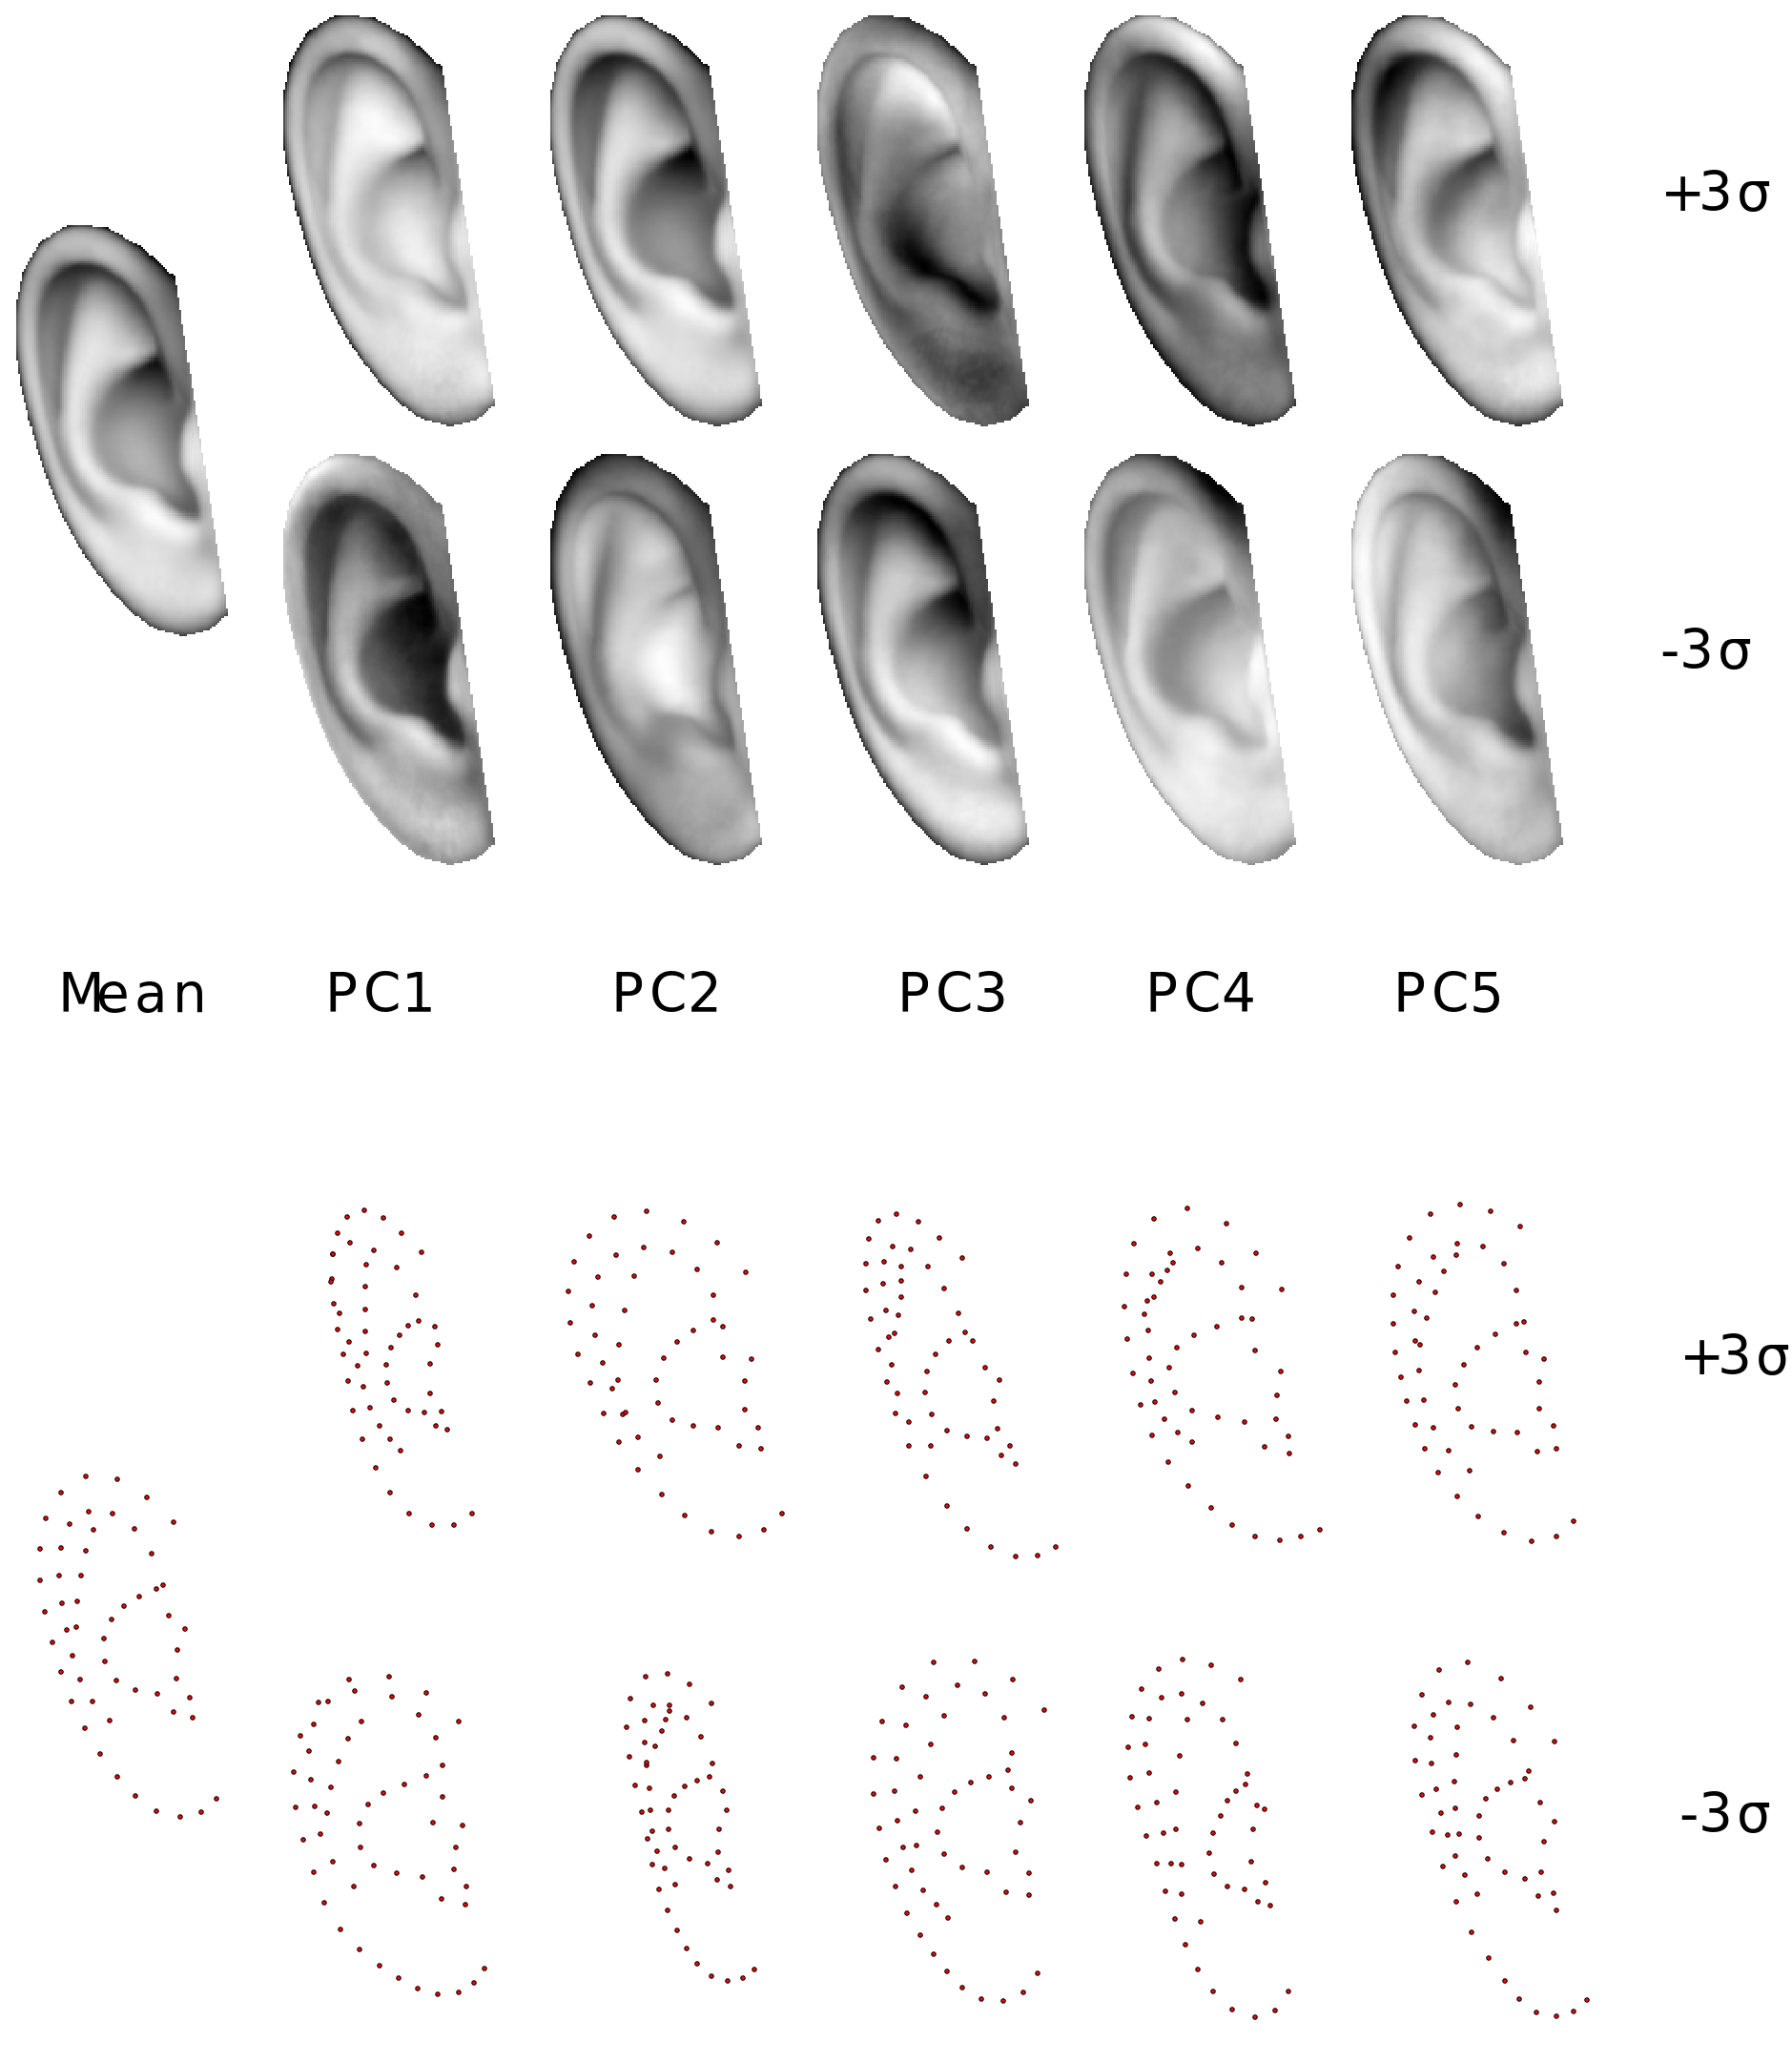
\includegraphics[width=\columnwidth]{resources/Ear_Deformable_Model/models/AAM_model}
    \caption{Exemplar statistical shape and appearance model of human ear. The figure visualises the first five principal components variation in both models. Appearance model is created with pixel intensity for better visualisation.}
    \label{fig:aam_model}
\end{figure}


%$\bullet$ The abundance of complex visual data, spread mostly through the Internet via web services such as %Youtube, Flickr and Google Images. The latter has led to the development of large databases of %``in-the-wild'' images of human faces and bodies~\cite{Belhumeur2011, Le2012, Zhu2012, Burgos2013, %sagonas_iccv_300w_2013}.

%$\bullet$ The development of powerful visual features, able to describe objects in a robust manner (e.g. $Image Gradient Orientation (IGO)~\cite{tzimiropoulos2012subspace}, Scale Invariant Feature Transforms $(SIFT)~\cite{lowe1999object}, Histogram of Oriented Gradients (HOG)~\cite{Dalal2005} and recently Deep $Convolutional Neural Networks (DCNN)~\cite{sermanet2013overfeat}), as well as generative and discriminative $methodologies for learning deformable models. 


%In this paper, we extend the application of SDMs to human ears, for which we show that sensible and %powerful models can be constructed. Given the great properties demonstrated by the ear for human %identification, we study the feasibility of building statistical deformable models of ears that have robust %and accurate performance with images captured under unconstrained conditions (commonly referred to as %``in-the-wild"). We employ the widely-used state-of-the-art holistic and patch-based Active Appearance %Models (AAMs)~\cite{Cootes2001, Matthews2004, Tzimiropoulos2014, antonakos2015feature}. Meanwhile, dataset %consists of 605 in-the-wild images, with careful annotation, are collected for ear AAM modelling.

The other contribution of the paper is the collection of a new ``in-the-wild'' database suitable for ear
verification and recognition. The collected database consists of 231 subjects with 2058 ``in-the-wild'' images. We conduct extensive experimental comparisons in the newly collected database using various handcrafted features such as Image Gradient Orientation (IGO)~\cite{tzimiropoulos2012subspace}, Scale Invariant Feature Transforms (SIFT)~\cite{lowe1999object}, Histogram of Oriented Gradients (HOG)~\cite{Dalal2005}, as well as learned deep convolutional features~\cite{sermanet2013overfeat}. Finally, we compare the effect of alignment in ear recognition/verification.
Summarising, the contributions proposed in this paper are:
    \begin{itemize}
    \item We present the first annotated ``in-the-wild'' database of images of ears (605 images in total) with regards to 55 landmarks. We provide the database publicly available.
    \item We conduct an extensive comparison between various discriminant and generative methodologies for ear landmark localisation ``in-the-wild''.
    \item We collect a large database of ears ``in-the-wild'' for ear recognition/verification and we conduct an extensive experimental comparison. 
    \end{itemize}

% To the best of our knowledge this is the first methodology which can create a dense statistical model for AAM which can operate in ``in-the-wild''.





% -----------------------------------------------------------------------------------------------------------------------



\section{Existing Databases}

In the following we briefly review the available databases for ear recognition and argue for a collection of a new one ``in-the-wild'' database for ear alignment and one for ear recognition/verification ``in-the-wild''. 
The list of the most popular ear databases includes the following database UND-Collection E~\cite{UNDE}, EUBEAR~\cite{raposo2011ubear}, IIT~\cite{kumar2012automated}, WPUTEDB~\cite{frejlichowski2010west} and ScFace~\cite{grgic2011scface}), most of which have been captured under controlled laboratory conditions or lack of annotations. In particular, 

\noindent\textbf{UND Databases Collection E} includes 464 right profiled ear images from 114 identities, from which 3 to 9 images are taken for each person in days with various pose and illumination conditions.

\noindent\textbf{WPUTEDB} introduces 3348 images of 421 subjects each having 4 to 12 images taken under controlled environments~\cite{frejlichowski2010west}. Various indoor lighting conditions, occlusion by hair and accessories, and slightly angled positions are involved in this database to simulate ``in-the-wild'' condition but still very limited to specific scenario. 

\noindent\textbf{IIT Delhi} database contains 125 subjects where each has 3 to 6 images taken in grayscale. Images are taken in indoor condition with limited lighting variation. No or occasionally occlusion and pose variation occurred.

\noindent\textbf{UBEAR} dataset involved 126 subjects with an average 35 images corresponding to each subject. Lighting conditions, pose variations and occlusions are all applied to this database. But images are collected from indoor video therefore the with-in class variation is quite limited.

Note that all datasets above are collected under controlled environment and none, to the best of our knowledge, has been annotated with regards to landmarks. Furthermore, as we will show in the experimental result section, in WPUTEDB database the area around the ear contains very discriminative information. This is an indication that the data have been collected within small time intervals. In this paper, we make a significant step further and collect and annotate databases of ears ``in-the-wild''.  Furthermore, we made an effort so that the ear samples for each person have been taken with considerable time interval. 

To the best of our knowledge the only ear database that has been collected ``in-the-wild'' is the one presented in~\cite{emervsivc2015ear}, which contains a very limited amount of subjects (only 16).

\section{``In-the-wild'' Ear database}
\label{label:ear_db}
We collected two sets of ear images ``in-the-wild''\footnote{\label{foot:annotations_ear}Both Collection A and B are publicly available in http://www.ibug.doc.ic.ac.uk/resources/ibug-ears.}. The first was used for  statistical deformable model construction, while the latter was used for ear verification and recognition ``in-the-wild''.

\begin{figure}
    \centering
    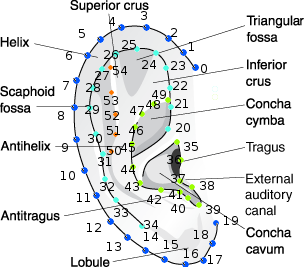
\includegraphics[width=\columnwidth]{resources/Ear_Deformable_Model/pinna} \\
    \newcommand{\flowh}{0.22\columnwidth}
    % \newcommand{\flowhh}{0.2\columnwidth}
    \newcommand{\flowhhh}{0.21\columnwidth}
    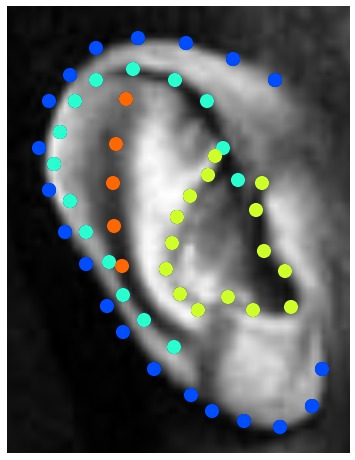
\includegraphics[height=\flowh]{resources/Ear_Deformable_Model/dbs/db_1}
    \hfill
    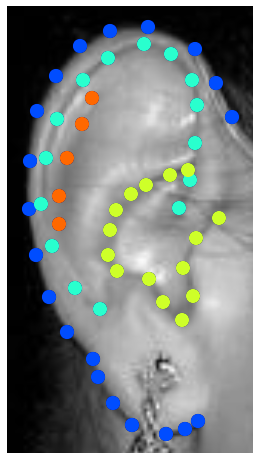
\includegraphics[height=\flowh]{resources/Ear_Deformable_Model/dbs/db_2}
    \hfill
    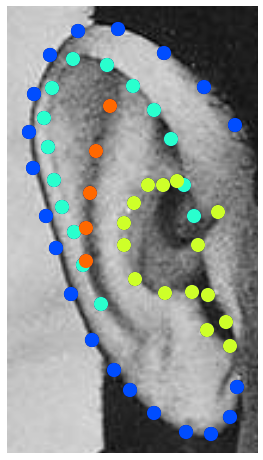
\includegraphics[height=\flowh]{resources/Ear_Deformable_Model/dbs/db_3}
    \hfill
    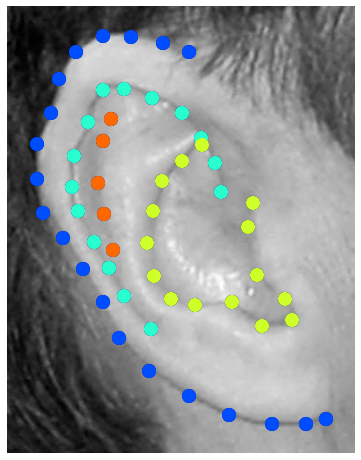
\includegraphics[height=\flowh]{resources/Ear_Deformable_Model/dbs/db_4} 
    \hfill
    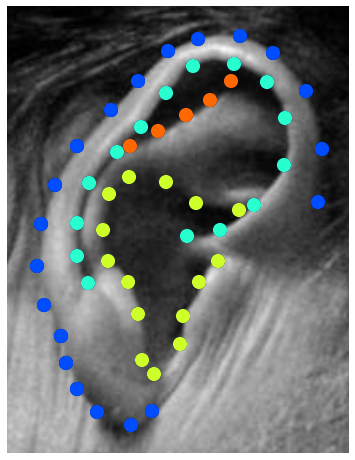
\includegraphics[height=\flowh]{resources/Ear_Deformable_Model/dbs/db_5}
    \hfill
    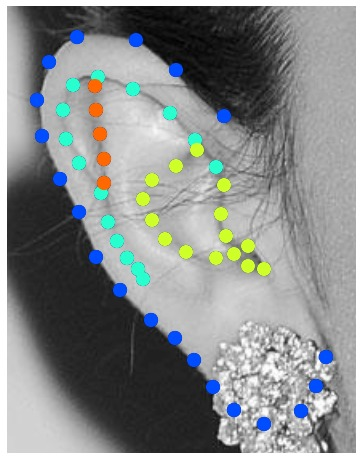
\includegraphics[height=\flowh]{resources/Ear_Deformable_Model/dbs/db_6}
    \\
    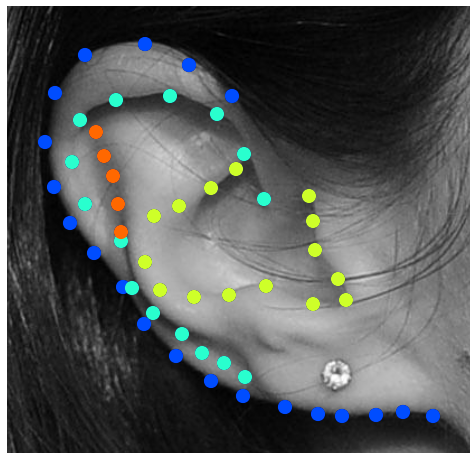
\includegraphics[height=\flowhhh]{resources/Ear_Deformable_Model/dbs/db_7}
    \hfill
    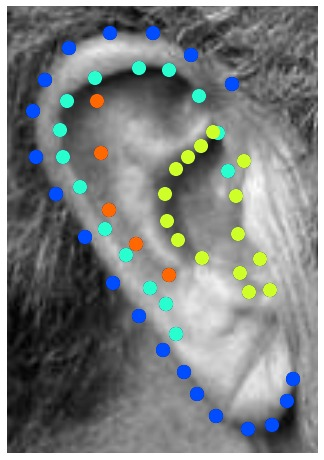
\includegraphics[height=\flowhhh]{resources/Ear_Deformable_Model/dbs/db_8} 
    \hfill
    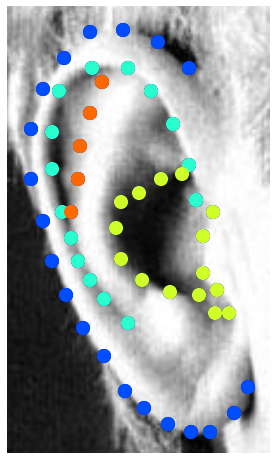
\includegraphics[height=\flowhhh]{resources/Ear_Deformable_Model/dbs/db_9}
    \hfill
    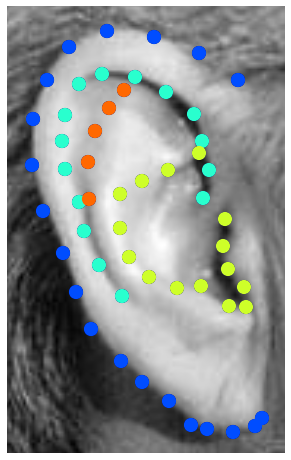
\includegraphics[height=\flowhhh]{resources/Ear_Deformable_Model/dbs/db_10}
    \hfill
    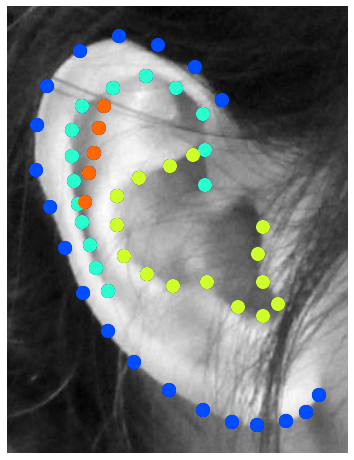
\includegraphics[height=\flowhhh]{resources/Ear_Deformable_Model/dbs/db_11}
    \hfill
    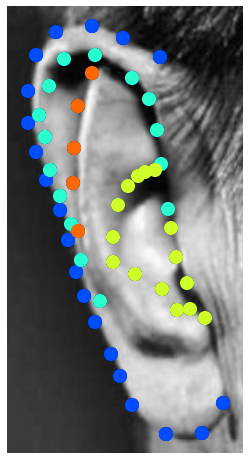
\includegraphics[height=\flowhhh]{resources/Ear_Deformable_Model/dbs/db_12}
    \caption{Example of the annotated 55 landmarks on ears. Ascending helix (0-3), descending helix (4-7), helix (8-13), ear lobe (14-19), ascending inner helix (20-24), descending inner helix (25-28), inner helix (29-34), tragus (35-38), canal (39), antitragus (40-42), concha (43-46), inferio crus (47-49) and supperio crus (50-54).}
    \label{fig:db_example}
\end{figure}

\textbf{Collection A} consists of 605 ear images ``in-the-wild'' collected from Google Images with no specific identity (by searching using the ear related tags). Each is manually annotated with 55 landmark points. Examples of such annotated images and the anatomy of pinna is shown in figure~\ref{fig:db_example}. The semantic meaning of the 55 landmarks are: ascending helix (0-3), descending helix (4-7), helix (8-13), ear lobe (14-19), ascending inner helix (20-24), descending inner helix (25-28), inner helix (29-34), tragus (35-38), canal (39), antitragus (40-42), concha (43-46), inferio crus (47-49) and supperio crus (50-54). We randomly split the images into two disjoint sets for training (500) and testing (105). The purpose of Collection A is to build statistical deformable models with unconstrained ear samples.

\textbf{Collection B} contains 2058 images contains 231 identity-labelled subjects collected from VGG database~\cite{Parkhi15}, which contains more than one million images of celebrities with only identity labels. As the purpose of VGG database was face recognition ``in-the-wild'', we had to manual select images were ears are visible (not fully occluded) and furthermore there bounding box could be 
generated by a simple HoG Support Vector Machine (SVM)~\cite{Dalal2005}  ear detector (trained on collection A). Exemplar collected ear images are shown in Figure~\ref{fig:db_example} that images are under challenging environment such as heavily posed angle, significant lighting variations, notable occlusions, variant resolutions, and significant ageing. It is so far, to the best of our knowledge, the largest ear in-the-wild databases. The most related database is~\cite{emervsivc2015ear}, which contains only 16 subjects. 
%Moreover, rather than cropping images to ears as general ear database did, we maintained the original in-the-wild images with ear bounding box provided. As mentioned in introduction, face verification accuracy drops significantly on profiled faces, while ears are relatively clear in this case. So we kept original images in our database where faces are all posed at 30-150 degrees from frontal. With fused information from ears, we can also boost face verification accuracy at posed senario.
\label{600EW}

Upon acceptance of the paper, both databases will be made available to the research community.

%%%%%%%%%%%%%%%%%%%%%%%%%%%%%%%%%%%%%%%%%%%%%%%%%%%%%%%%%%%%%%%%%%%%%%%%%%%%%%%%




\section{Holistic and Patch-based Statistical Deformable Models}

We have applied many state-of-the-art statistical deformable models for ear landmark localisation. The methodologies includes Constrained Local Models (CLMs)~\cite{cristinacce2006feature}, Supervised Descent Method (SDM)~\cite{xiong2013supervised} and various Active Appearance Model (AAM) methods~\cite{Cootes2001, Matthews2004, Tzimiropoulos2014, antonakos2015feature}. In the following, we will focus on the general AAM architectures applied, since they were the top performing ones. The annotated ear dataset was used to  build two different kind of AAMs~\cite{Cootes2001, Matthews2004}: \emph{holistic}~\cite{ramnath2008increasing, Amberg2009, anderson2014using, antonakos2015feature} and \emph{patch-based}~\cite{Tzimiropoulos2014}. The difference between these two models is on the way that the appearance is represented, as well as the deformation model.


\subsection{Holistic Active Appearance Model}
\label{sec:bg_aam_ear}
AAM method consists of a linear statistical model of the shape and appearance of an object. During fitting, they aim to minimise the appearance reconstruction error with respect to the parameters of the shape and appearance models. Initially it was proposed to optimise their cost function using regression~\cite{Cootes2001}. Later, it was also shown that they can achieve state-of-the-art performance by employing the Gauss-Newton optimisation~\cite{Matthews2004,antonakos2015feature}.

\noindent\textbf{Shape Model}
A shape vector is defined by concatenating the coordinates of its landmarks. A shape model can be trained by applying Generalized Procrustes Analysis followed by Principal Component Analysis (PCA) on a set of training shapes. The shape model can then be used to generate shape instances with $N_L$ landmarks as
\begin{equation} 
\label{eq:shape_model_ear}
\bm{s_p}=\bm{\bar{s}}+\bm{U_S}\bm{p}
\end{equation} 
where a shape is represented as $\bm{s}=[x_1,y_1,..,x_{N_L},y_{N_L}]^T$, and $\bm{\bar{s}}$ is the mean shape, $\bm{p}$ are the shape parameters and $\bm{U_s}$ are the principal components matrix of dimension $\bm{U_S} \in \Re^{2N_L\times N_p}$, where $N_p$ represent the number of eigenvectors.

\noindent\textbf{Appearance Model}
\label{sec:appearance_model_ear}
A holistic appearance is defined as the values of the pixels that lie inside a shape $\bm{s}$. Similar to shape models, an appearance model is trained using PCA. Given the appearance eigenvectors $\bm{U_A}$, the mean appearance $\bm{\bar{a}}$ and a set of parameters $\bm{\lambda}$, a new appearance can be generated as 
\begin{equation} 
\label{eq:appearance_model}
\bm{a_\lambda}=\bm{\bar{a}}+\bm{U_A}\bm{\lambda}
\end{equation} 
where $\bm{a}$ denotes the vector of pixels that lie within a shape,  $\bm{\bar{a}}$ is the mean appearance, $\bm{\lambda}$ are the appearance parameters and $\bm{U_A}$ are the appearance principal components matrix of dimension $\bm{U_A} \in \Re^{N_A\times N_\lambda}$, where $N_\lambda$ represent the number of appearance eigenvectors and $N_A$ represented the length of eigenvector e.g. number of pixels within mean shape if single-channel appearance model considered. Note that the appearance can be represented by a handcrafted feature function (e.g. SIFT, HOG) or a learned feature (e.g. Dense CNN).

\noindent\textbf{Deformation Model} The deformation model of an AAM consists of a warp function $\mathcal{W}(\bm{p})$, which maps all the points $\bm{s_p}$ within a source shape defined by the shape parameters $p$ to their corresponding coordinates in a reference shape (commonly the mean shape $\bm{\bar{s}}$). This procedure is necessary in order to bring the appearance vectors of different images into correspondence. We employ the Piecewise Affine Warp, which performs the mapping based on the barycentric coordinates of the corresponding triangles between the two shapes that are extracted using Delaunay Triangulation.

\noindent\textbf{Fitting}
The aim of fitting is to minimise the $\ell_2^2$ norm between the warped appearance of an input image $\bm{T}(\mathcal{W}(\bm{p}))$ and the appearance model instance $\bm{a_\lambda}$ with respect to the shape and appearance parameters, i.e. 
\begin{equation} 
\label{eq:aamfitting_ear}
    \argmin_{\bm{p}, \bm{\lambda}}||\bm{T}(\mathcal{W}(\bm{p}))-\bm{\bar{a}}-\bm{U_A}\bm{\lambda}||^2
\end{equation}



\noindent\textbf{Inverse Compositional (IC) Algorithm} is an efficient gradient descend method that, in general, introduced an incremental warp, which composing with the current warp at each iteration as
\begin{equation}
\label{eq:composition}
\mathcal{W}(\bm{p})\leftarrow\mathcal{W}(\bm{p})\circ\mathcal{W}(\bm{\Delta p})^{-1}
\end{equation}
Thereby the cost function for inverse compositional algorithm are:
\begin{equation}
\label{eq:inversecomposition_ear}
\argmin_{\bm{\Delta p}, \bm{\lambda}}||\bm{T}(\mathcal{W}(\bm{p}))-\bm{\bar{a}}(\mathcal{W}(\bm{\Delta p}))-\bm{U_A}(\mathcal{W}(\bm{\Delta p}))\bm{\lambda}||^2
\end{equation}
where $\mathcal{W}(\bm{\Delta p})$ denotes incremental warp on template image. 
Applying first order Taylor expansion on equation~\ref{eq:inversecomposition_ear} gives:
\begin{equation}
\label{eq:forwardcompositiontaylor-ear}
\argmin_{\bm{\Delta p}, \bm{\lambda}}||\bm{T}(\mathcal{W}(\bm{p}))-\bm{\bar{a}}-\bm{U_A}\bm{\lambda}-\bm{J}|_{\bm{p}=\bm{0}}\bm{\Delta p}||^2
\end{equation}
where Jacobian term is defined as:
\begin{equation}
\label{eq:jacobian}
\bm{J}|_{\bm{p}=\bm{0}}=\nabla(\bm{\bar{a}}+\bm{U_A}\bm{\lambda})\frac{\partial \mathcal{W}}{\partial \bm{p}}|_{\bm{p}=\bm{0}}
\end{equation}

\begin{figure}
    \centering
    \newcommand{\flowh}{0.275\columnwidth}
    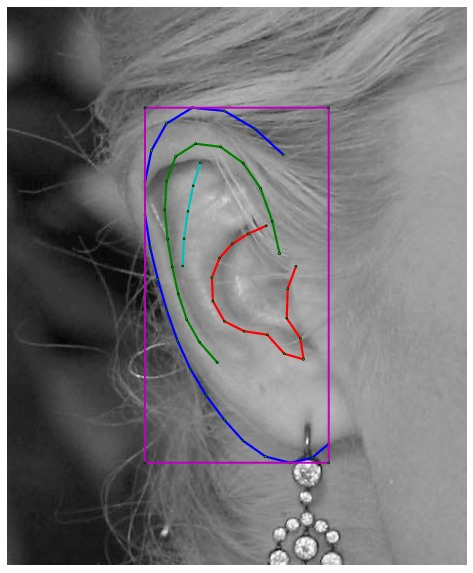
\includegraphics[height=\flowh]{resources/Ear_Deformable_Model/fittings/initial_0000}
    \hfill
    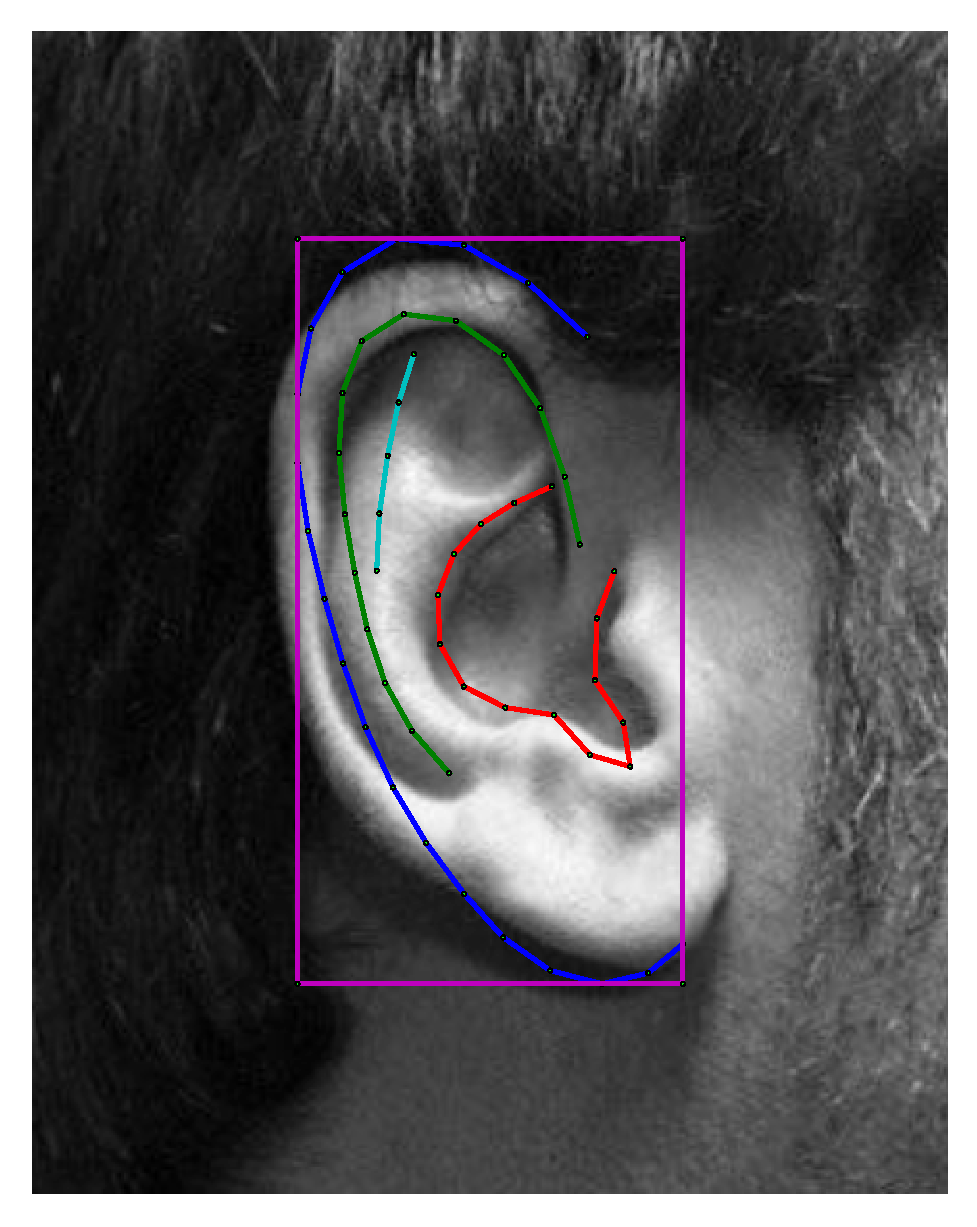
\includegraphics[height=\flowh]{resources/Ear_Deformable_Model/fittings/initial_0001}
    \hfill
    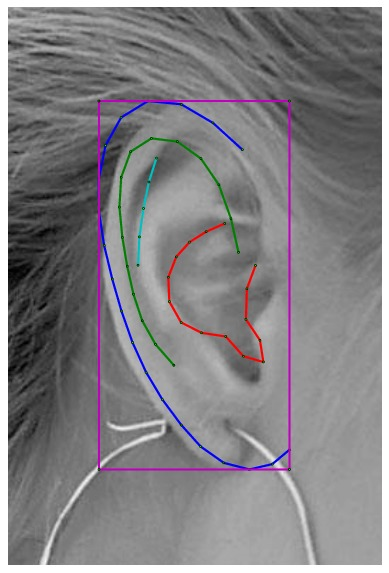
\includegraphics[height=\flowh]{resources/Ear_Deformable_Model/fittings/initial_0011}
    \hfill
    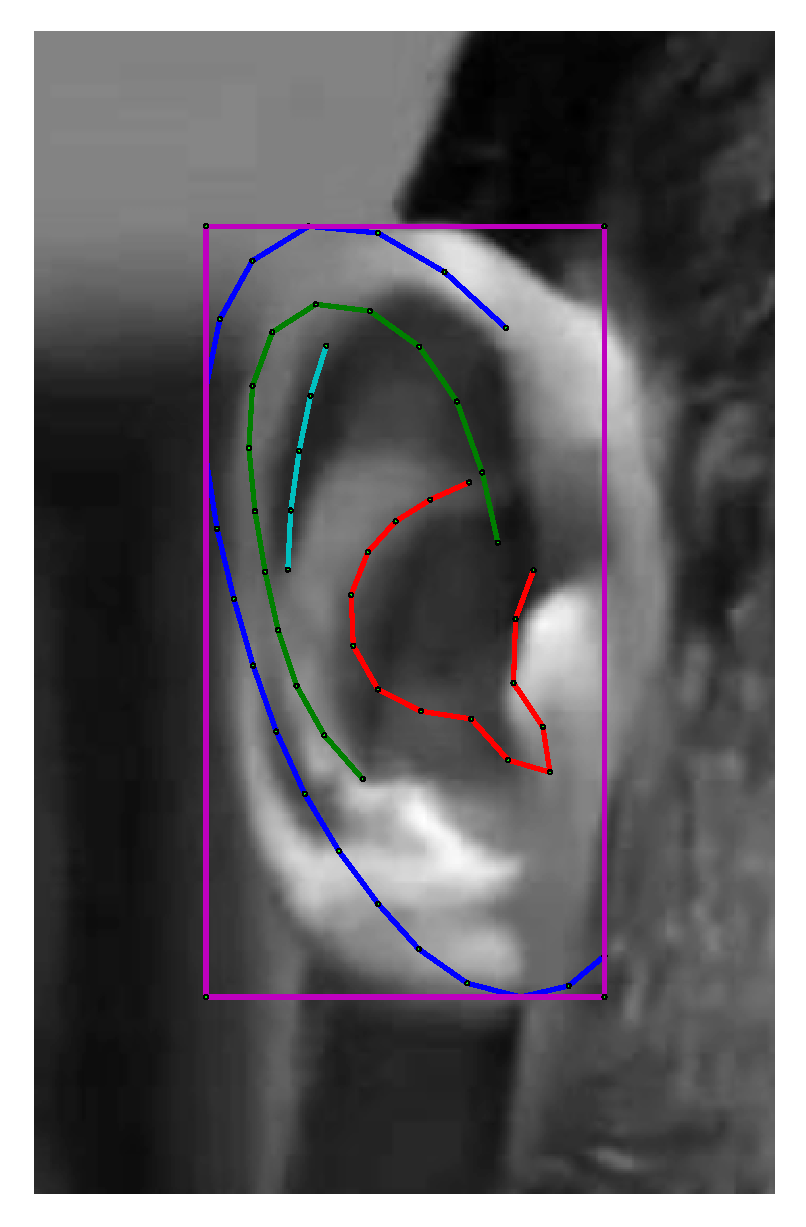
\includegraphics[height=\flowh]{resources/Ear_Deformable_Model/fittings/initial_0003}
    \hfill
    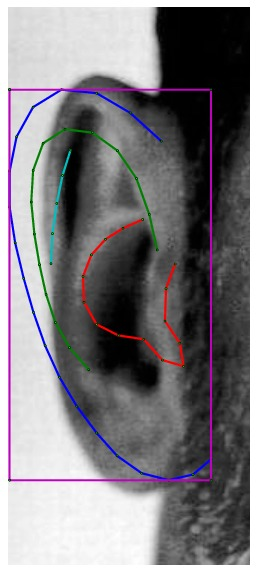
\includegraphics[height=\flowh]{resources/Ear_Deformable_Model/fittings/initial_0004}
    \hfill
    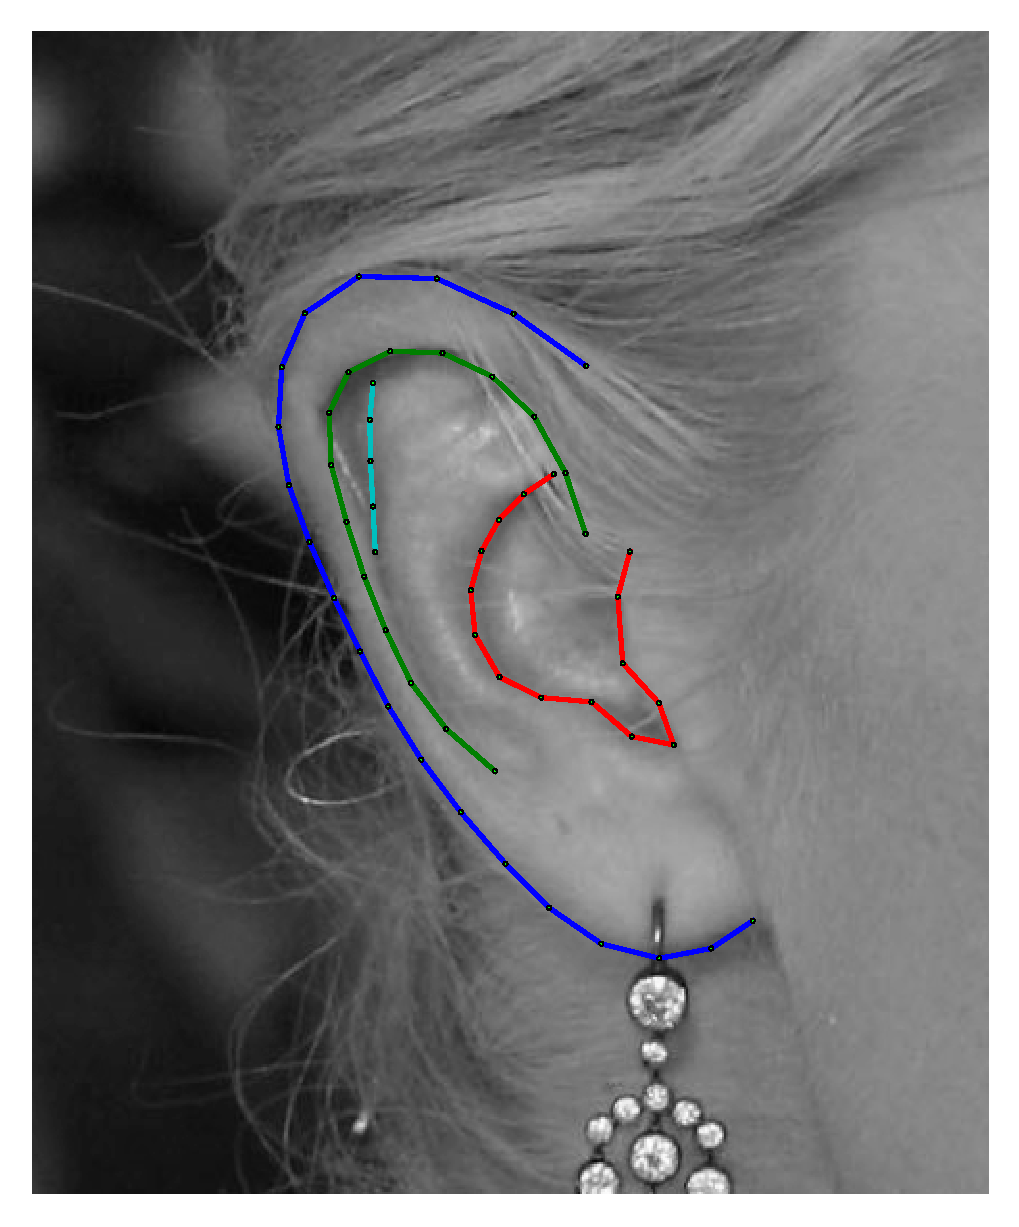
\includegraphics[height=\flowh]{resources/Ear_Deformable_Model/fittings/final_0000}
    \hfill
    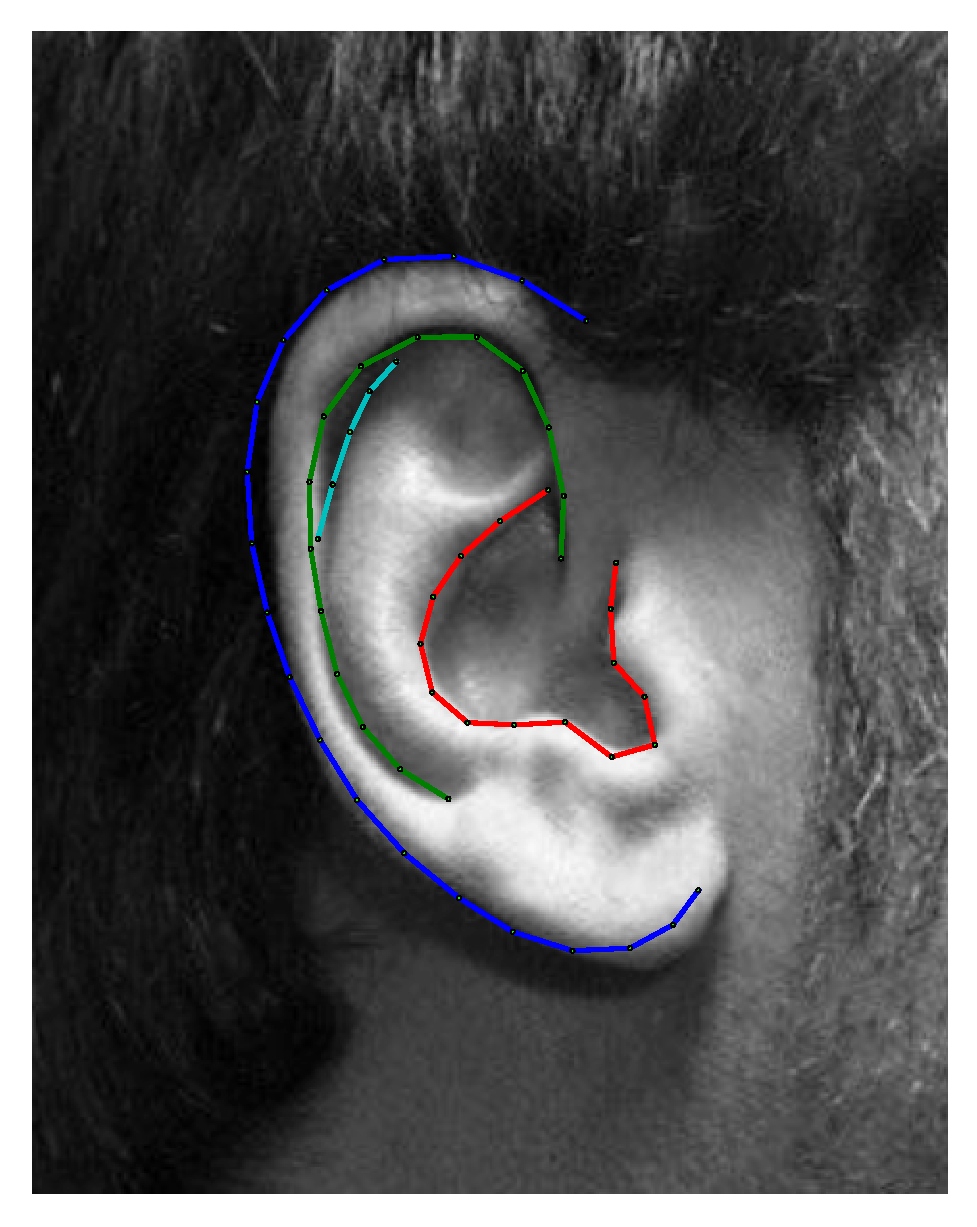
\includegraphics[height=\flowh]{resources/Ear_Deformable_Model/fittings/final_0001}
    \hfill
    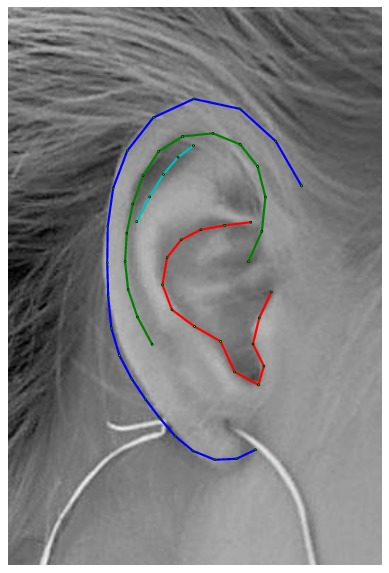
\includegraphics[height=\flowh]{resources/Ear_Deformable_Model/fittings/final_0011}
    \hfill
    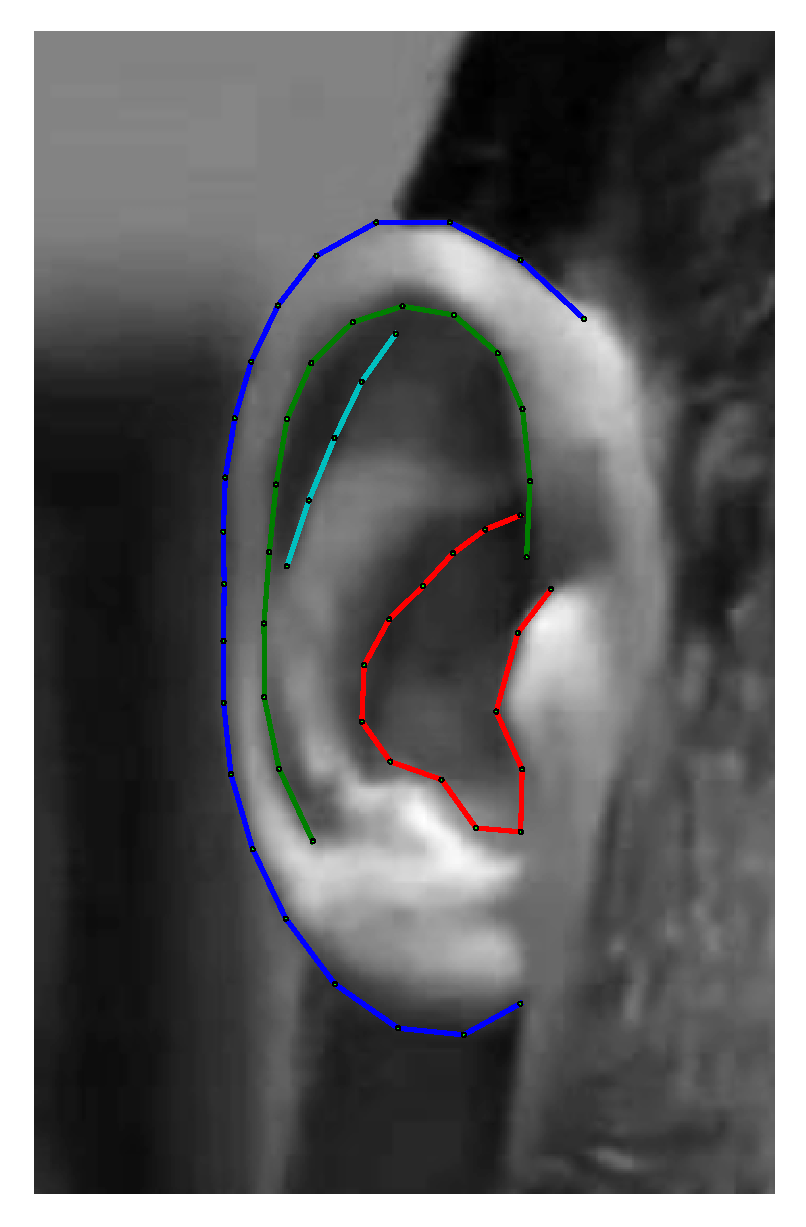
\includegraphics[height=\flowh]{resources/Ear_Deformable_Model/fittings/final_0003}
    \hfill
    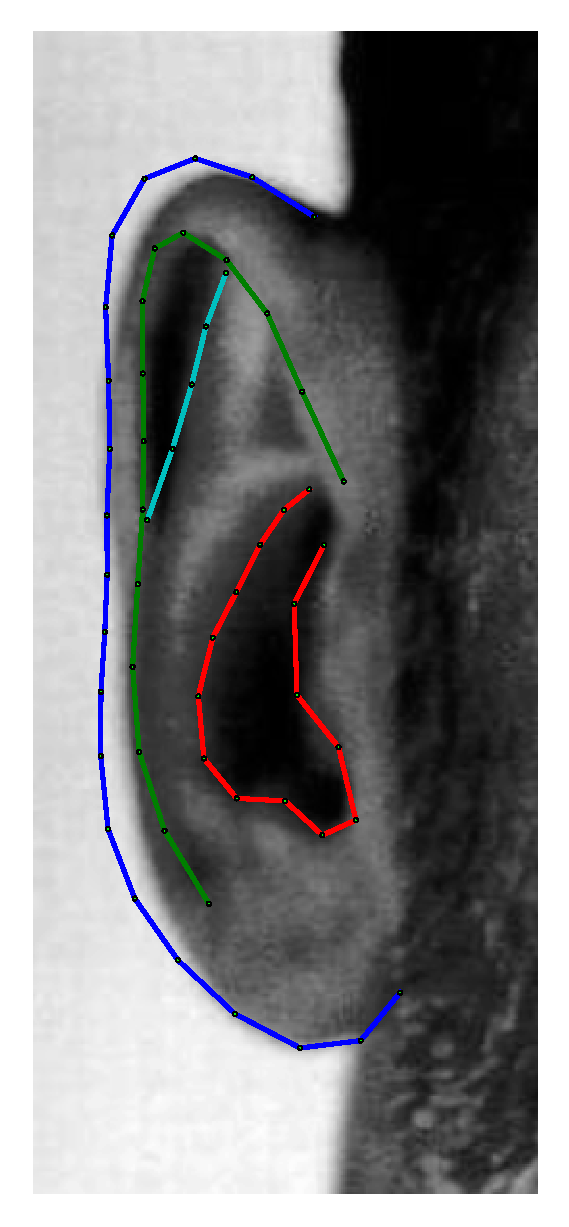
\includegraphics[height=\flowh]{resources/Ear_Deformable_Model/fittings/final_0004}
    \\
    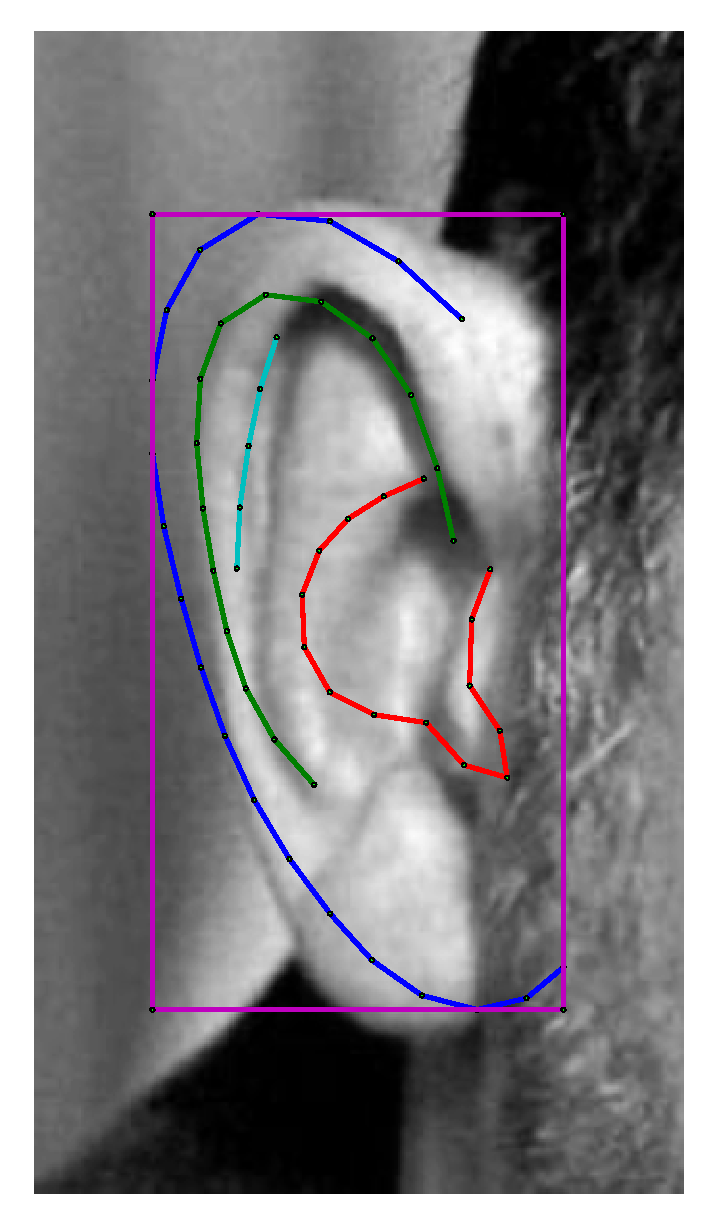
\includegraphics[height=\flowh]{resources/Ear_Deformable_Model/fittings/initial_0005}
    \hfill
    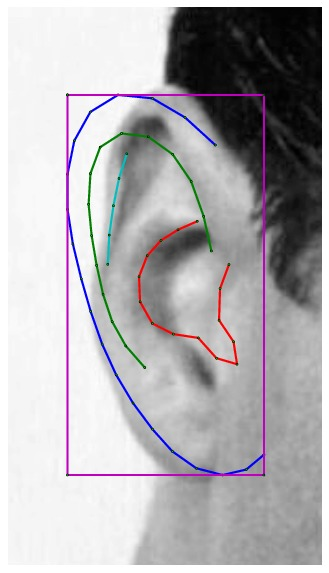
\includegraphics[height=\flowh]{resources/Ear_Deformable_Model/fittings/initial_0006}
    \hfill
    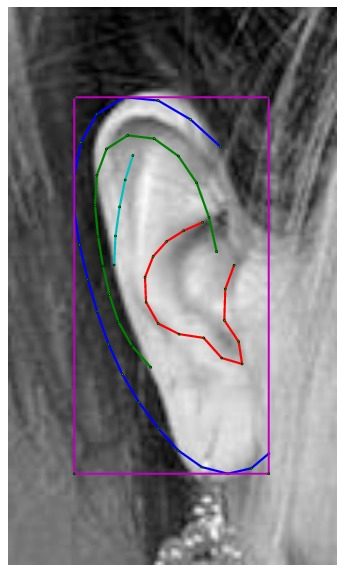
\includegraphics[height=\flowh]{resources/Ear_Deformable_Model/fittings/initial_0007}
    \hfill
    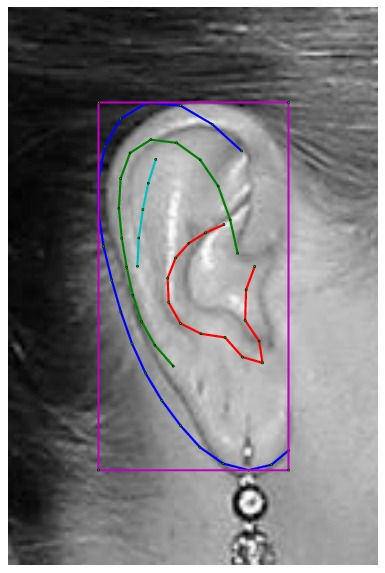
\includegraphics[height=\flowh]{resources/Ear_Deformable_Model/fittings/initial_0008}
    \hfill
    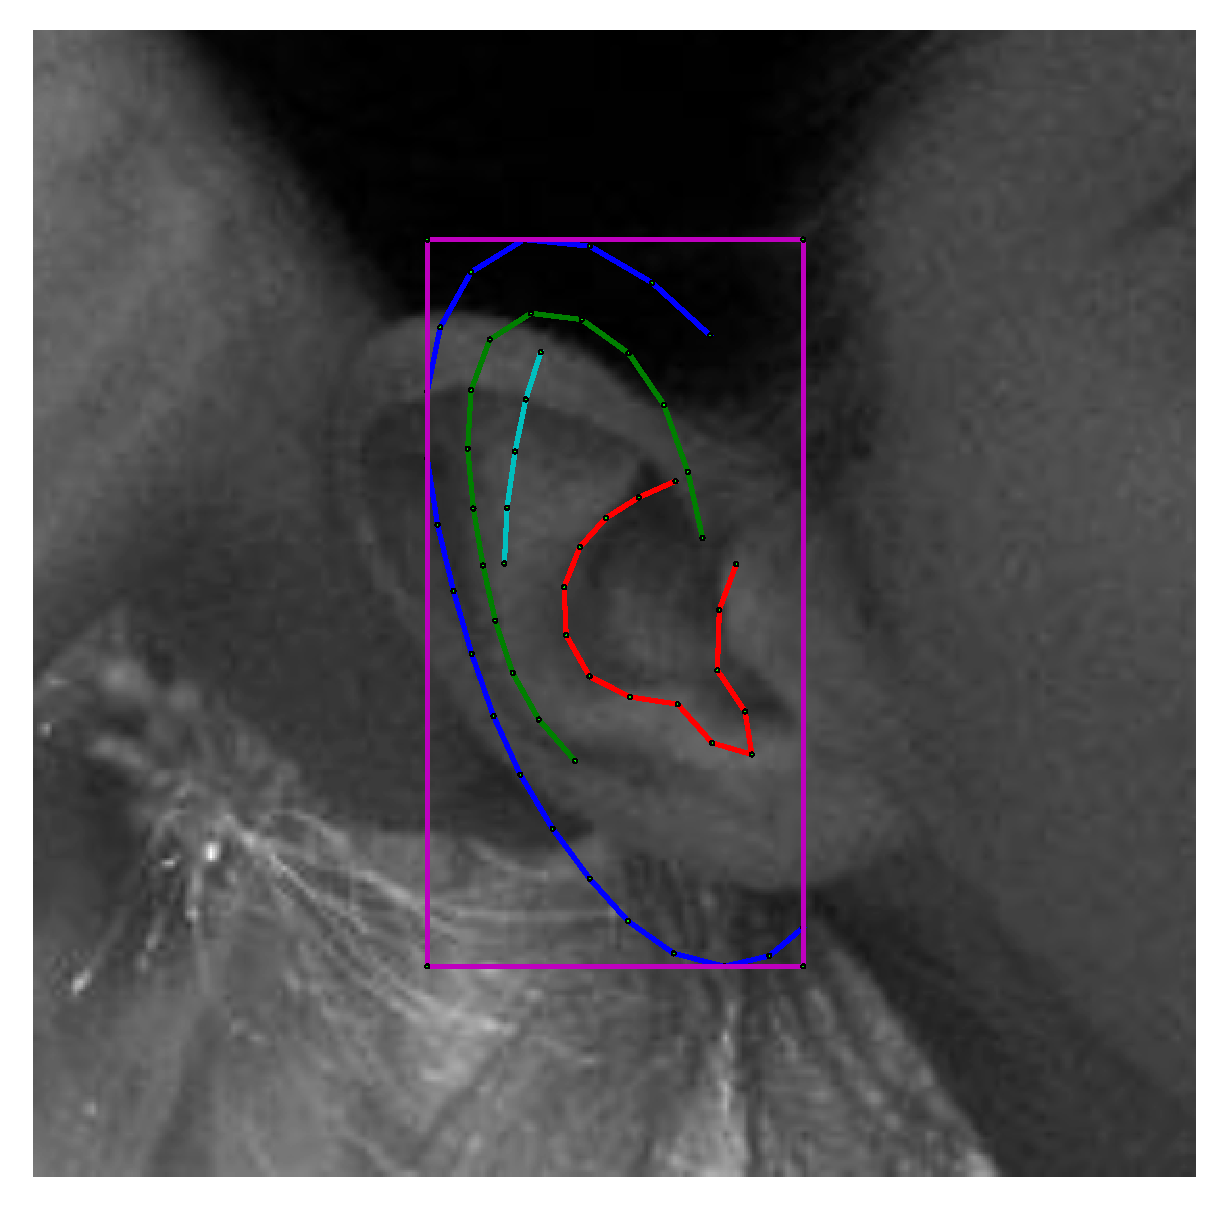
\includegraphics[height=\flowh]{resources/Ear_Deformable_Model/fittings/initial_0028}
    \hfill
    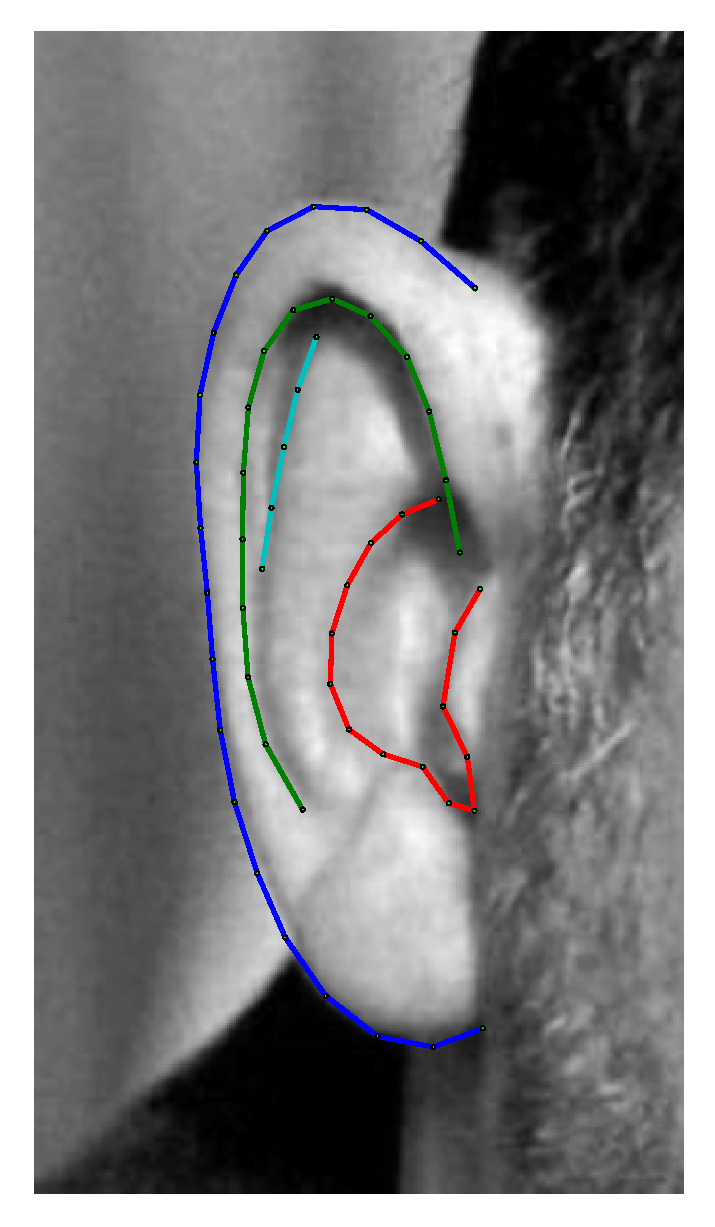
\includegraphics[height=\flowh]{resources/Ear_Deformable_Model/fittings/final_0005}
    \hfill
    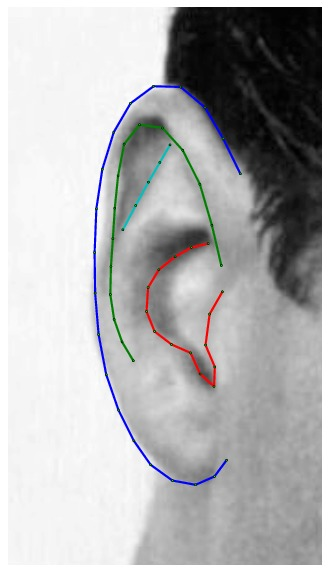
\includegraphics[height=\flowh]{resources/Ear_Deformable_Model/fittings/final_0006}
    \hfill
    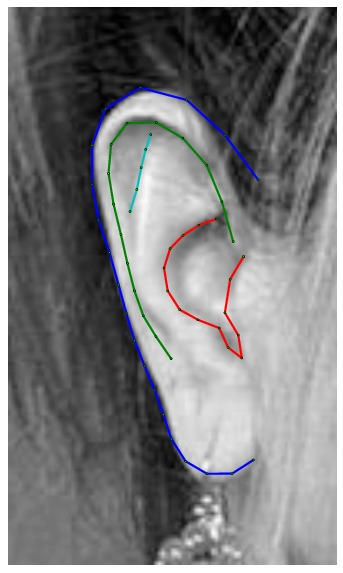
\includegraphics[height=\flowh]{resources/Ear_Deformable_Model/fittings/final_0007}
    \hfill
    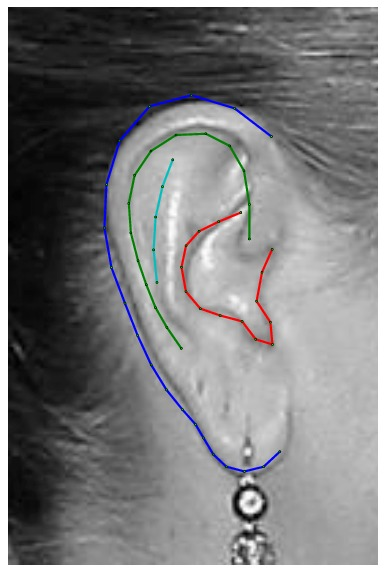
\includegraphics[height=\flowh]{resources/Ear_Deformable_Model/fittings/final_0008}
    \hfill
    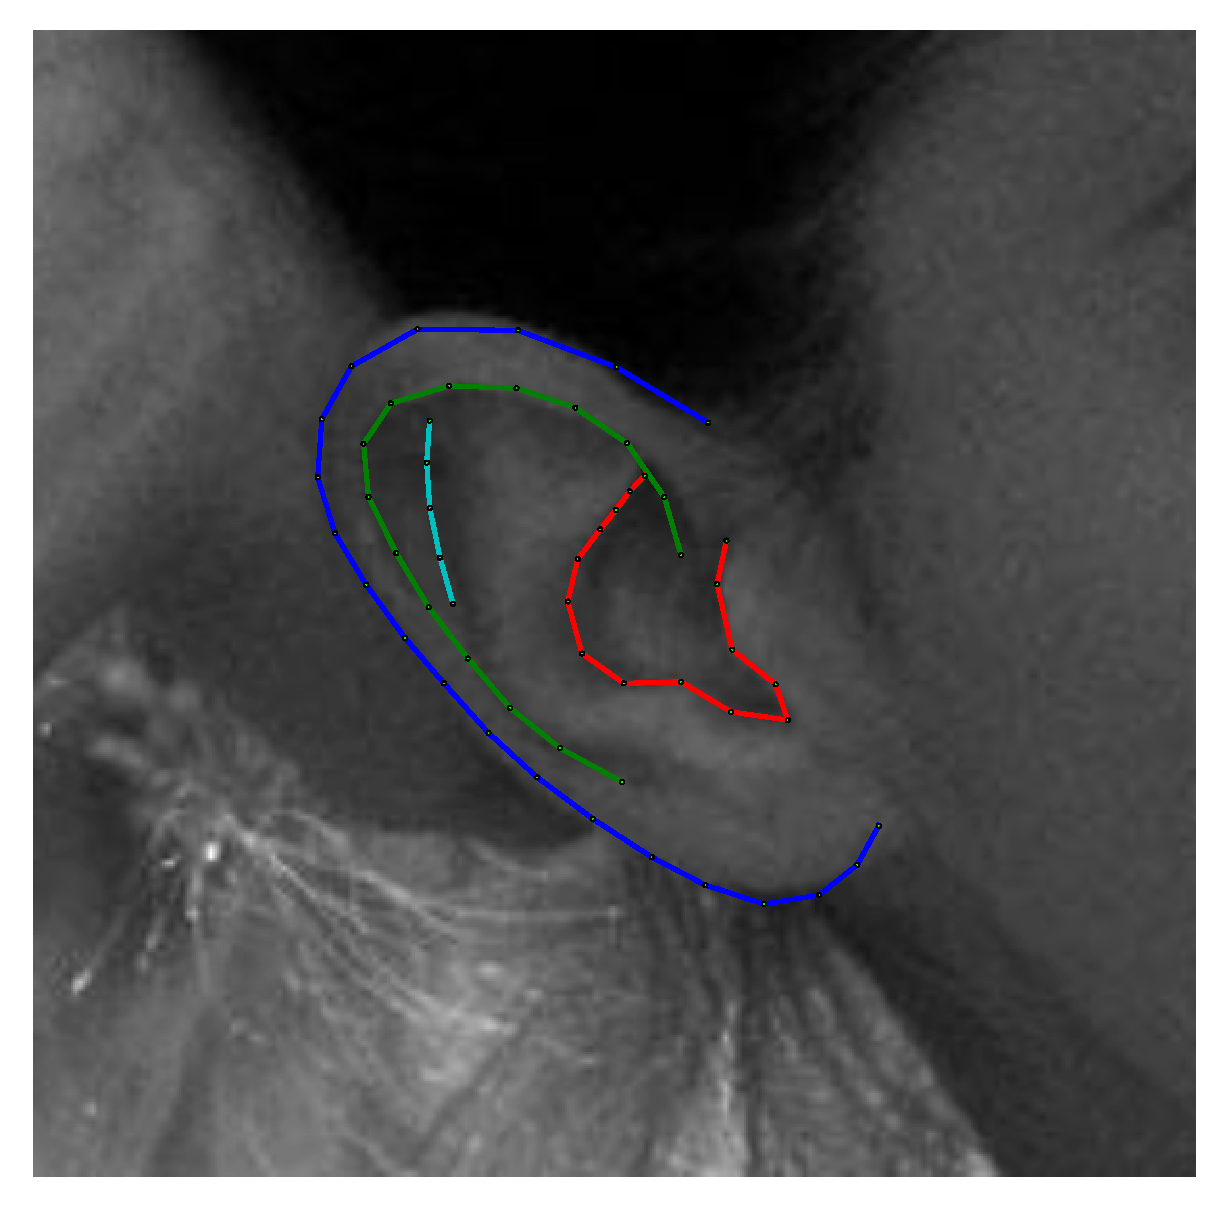
\includegraphics[height=\flowh]{resources/Ear_Deformable_Model/fittings/final_0028}
    \\
    \newcommand{\flowhh}{0.255\columnwidth}
    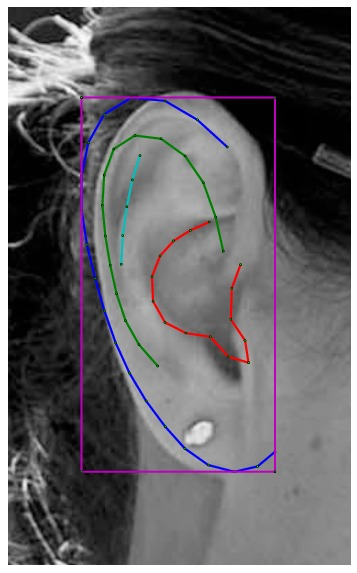
\includegraphics[height=\flowhh]{resources/Ear_Deformable_Model/fittings/initial_0012}
    \hfill
    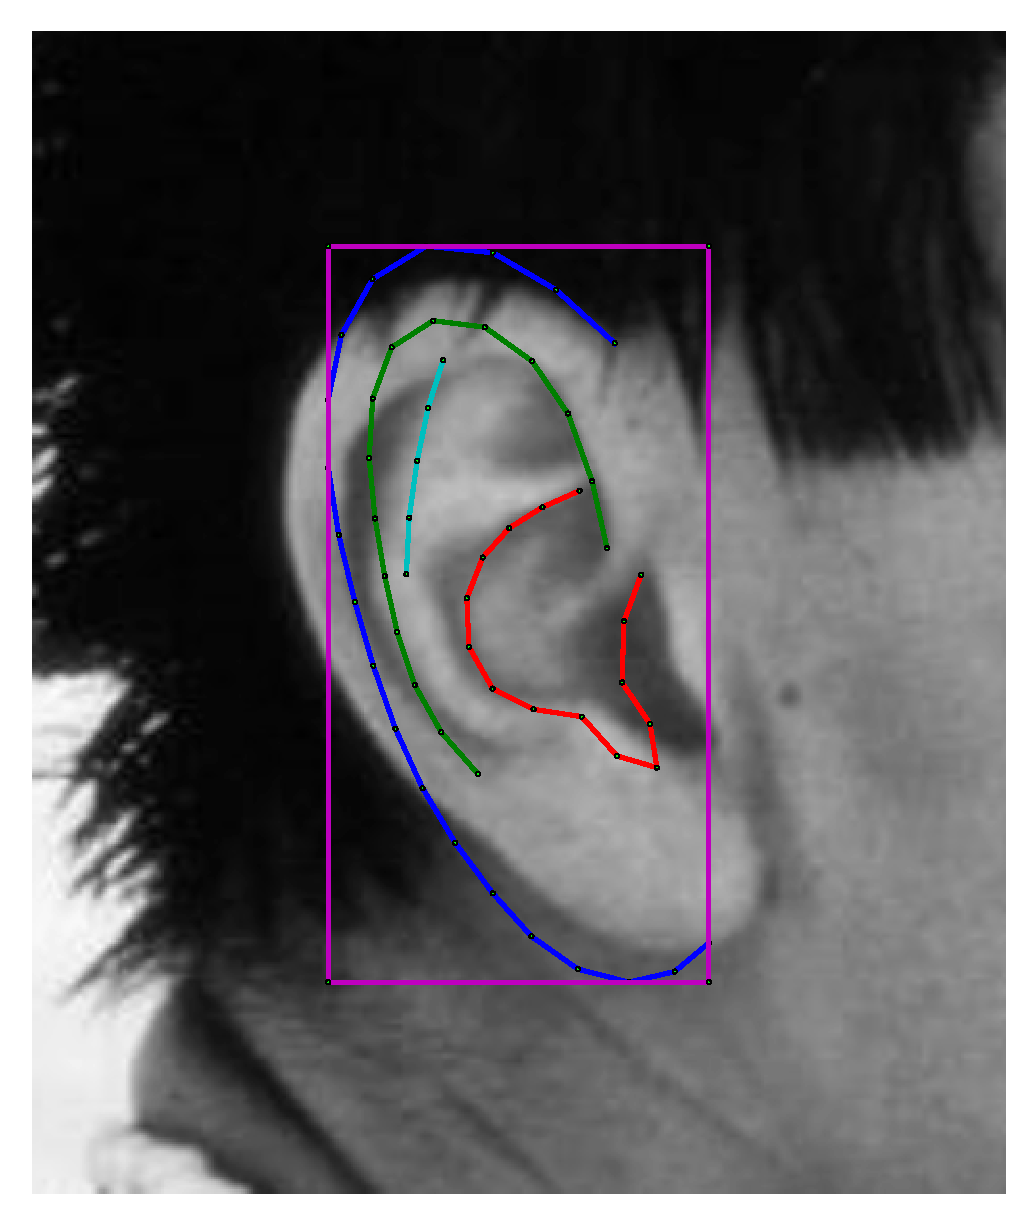
\includegraphics[height=\flowhh]{resources/Ear_Deformable_Model/fittings/initial_0022}
    \hfill
    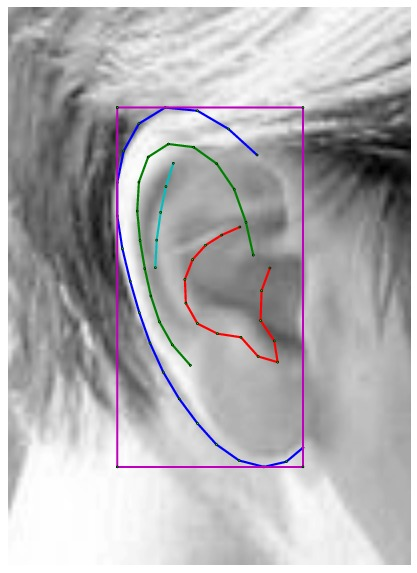
\includegraphics[height=\flowhh]{resources/Ear_Deformable_Model/fittings/initial_0023}
    \hfill
    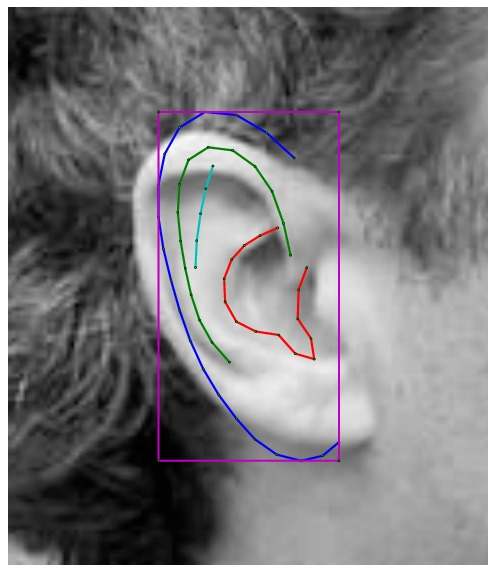
\includegraphics[height=\flowhh]{resources/Ear_Deformable_Model/fittings/initial_0015}
    \hfill
    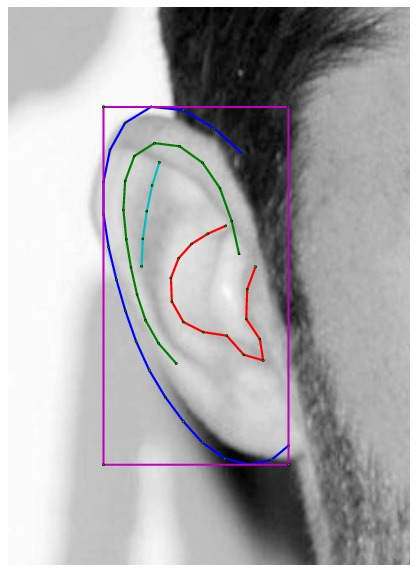
\includegraphics[height=\flowhh]{resources/Ear_Deformable_Model/fittings/initial_0024}
    \hfill
    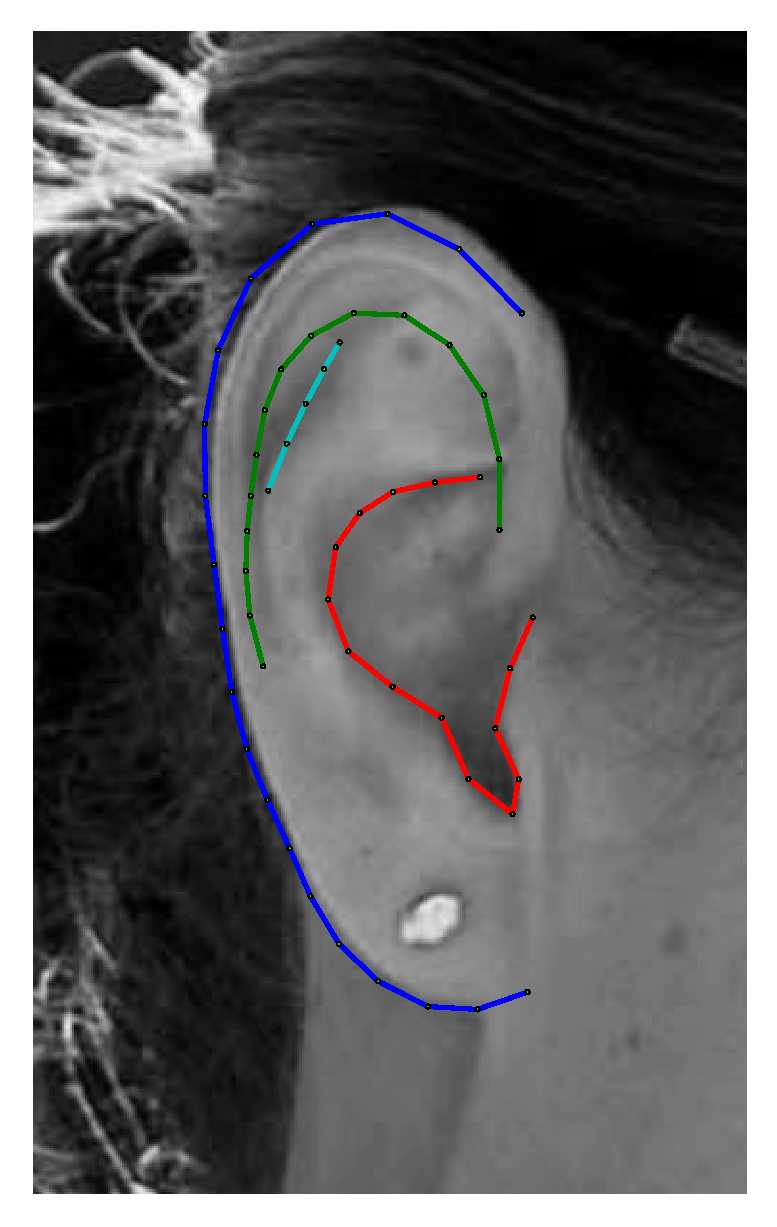
\includegraphics[height=\flowhh]{resources/Ear_Deformable_Model/fittings/final_0012}
    \hfill
    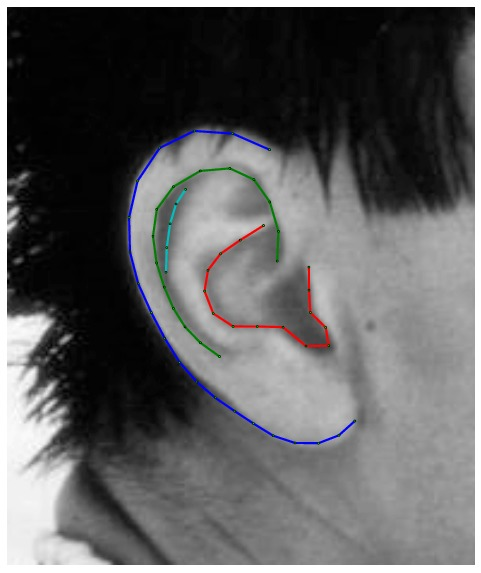
\includegraphics[height=\flowhh]{resources/Ear_Deformable_Model/fittings/final_0022}
    \hfill
    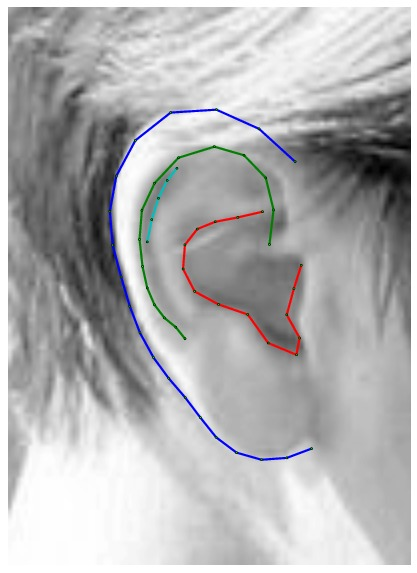
\includegraphics[height=\flowhh]{resources/Ear_Deformable_Model/fittings/final_0023}
    \hfill
    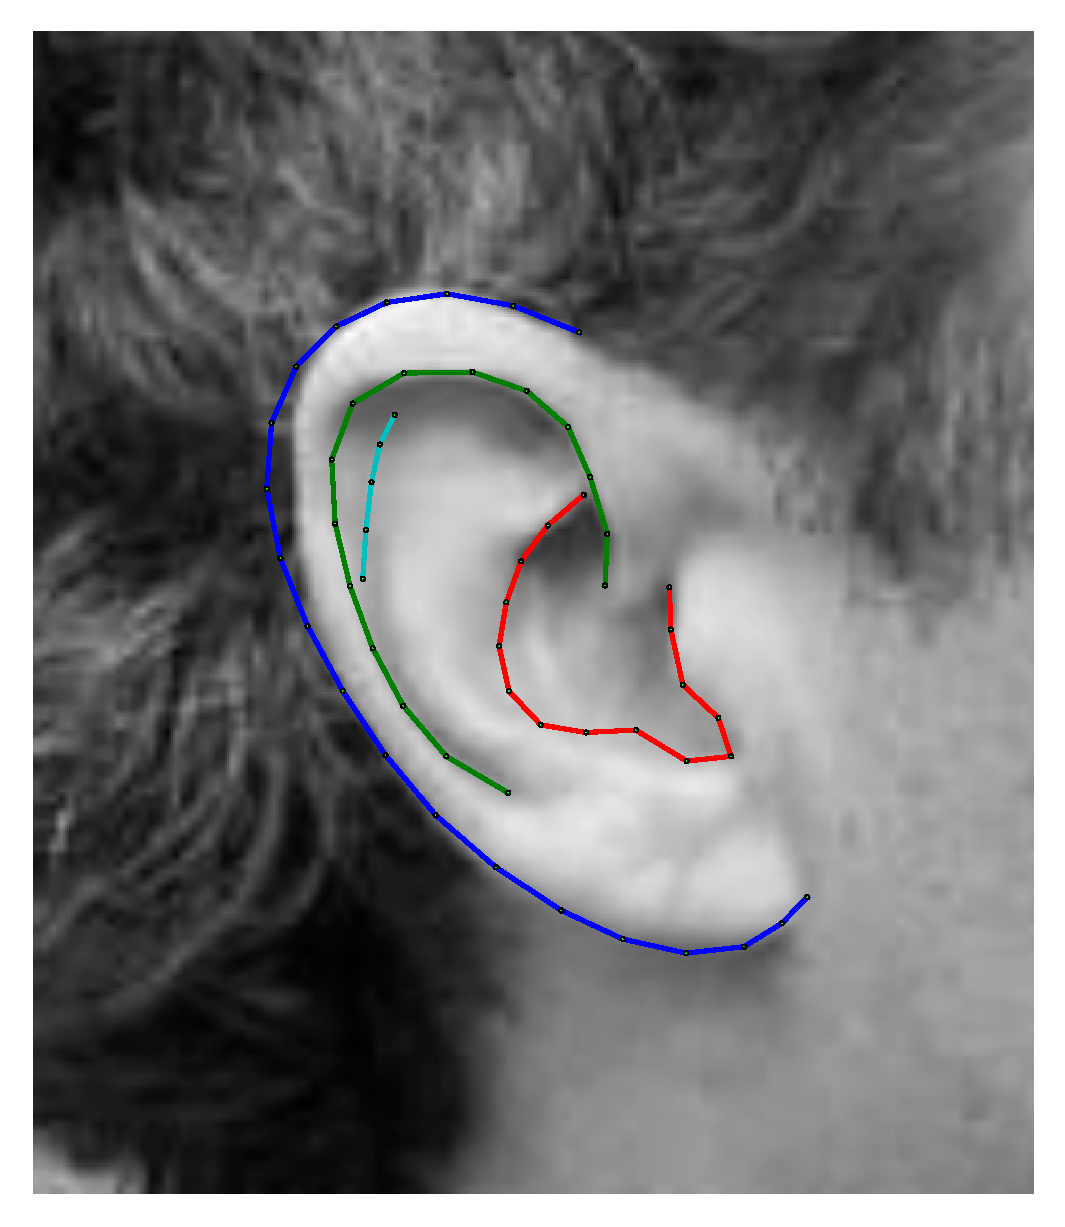
\includegraphics[height=\flowhh]{resources/Ear_Deformable_Model/fittings/final_0015}
    \hfill
    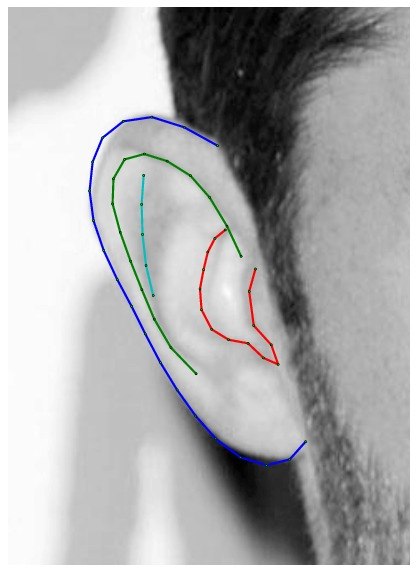
\includegraphics[height=\flowhh]{resources/Ear_Deformable_Model/fittings/final_0024}
    % \\
    % 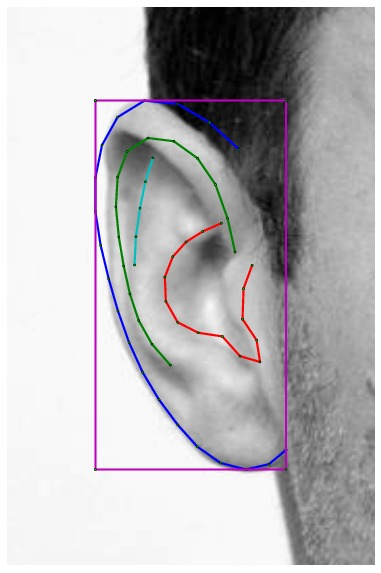
\includegraphics[height=\flowhh]{resources/Ear_Deformable_Model/fittings/initial_0025}
    % 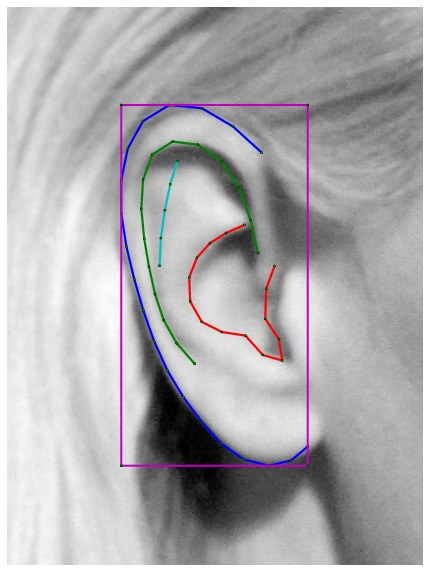
\includegraphics[height=\flowhh]{resources/Ear_Deformable_Model/fittings/initial_0010}
    % 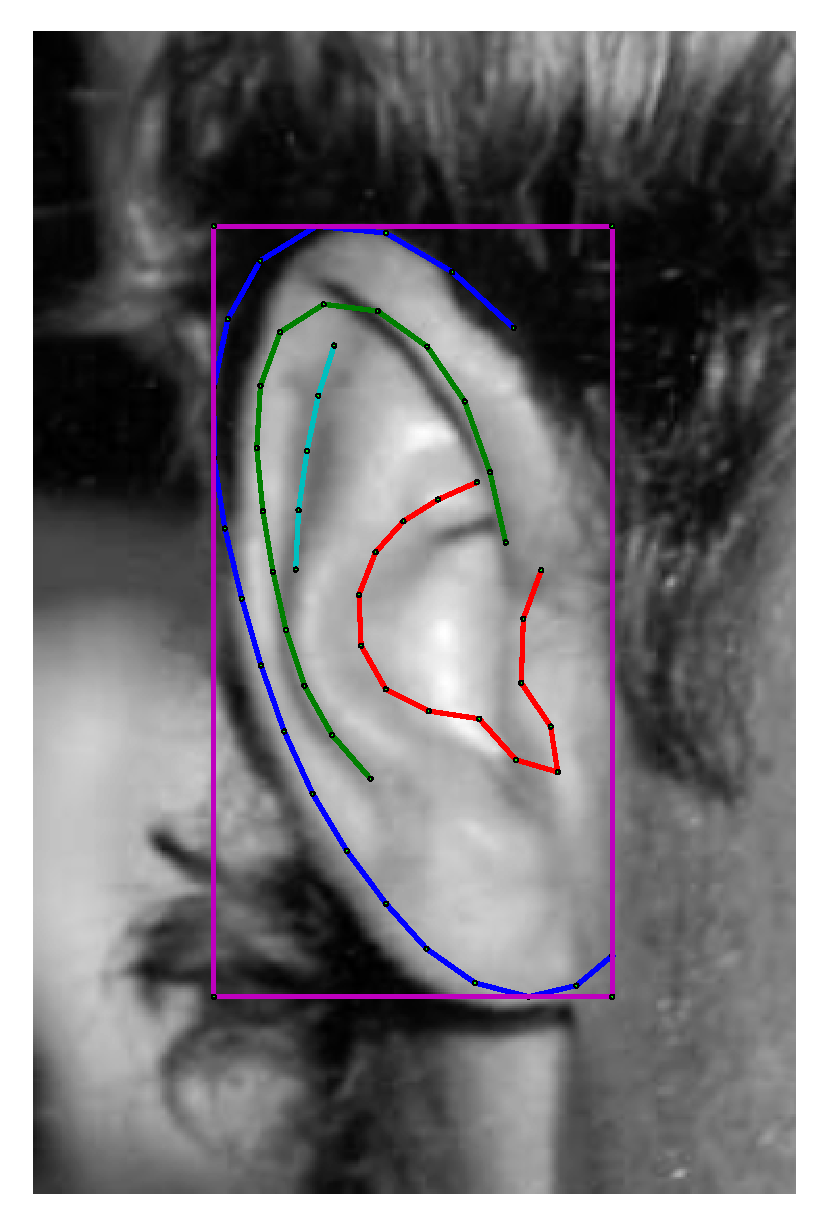
\includegraphics[height=\flowhh]{resources/Ear_Deformable_Model/fittings/initial_0027}
    % 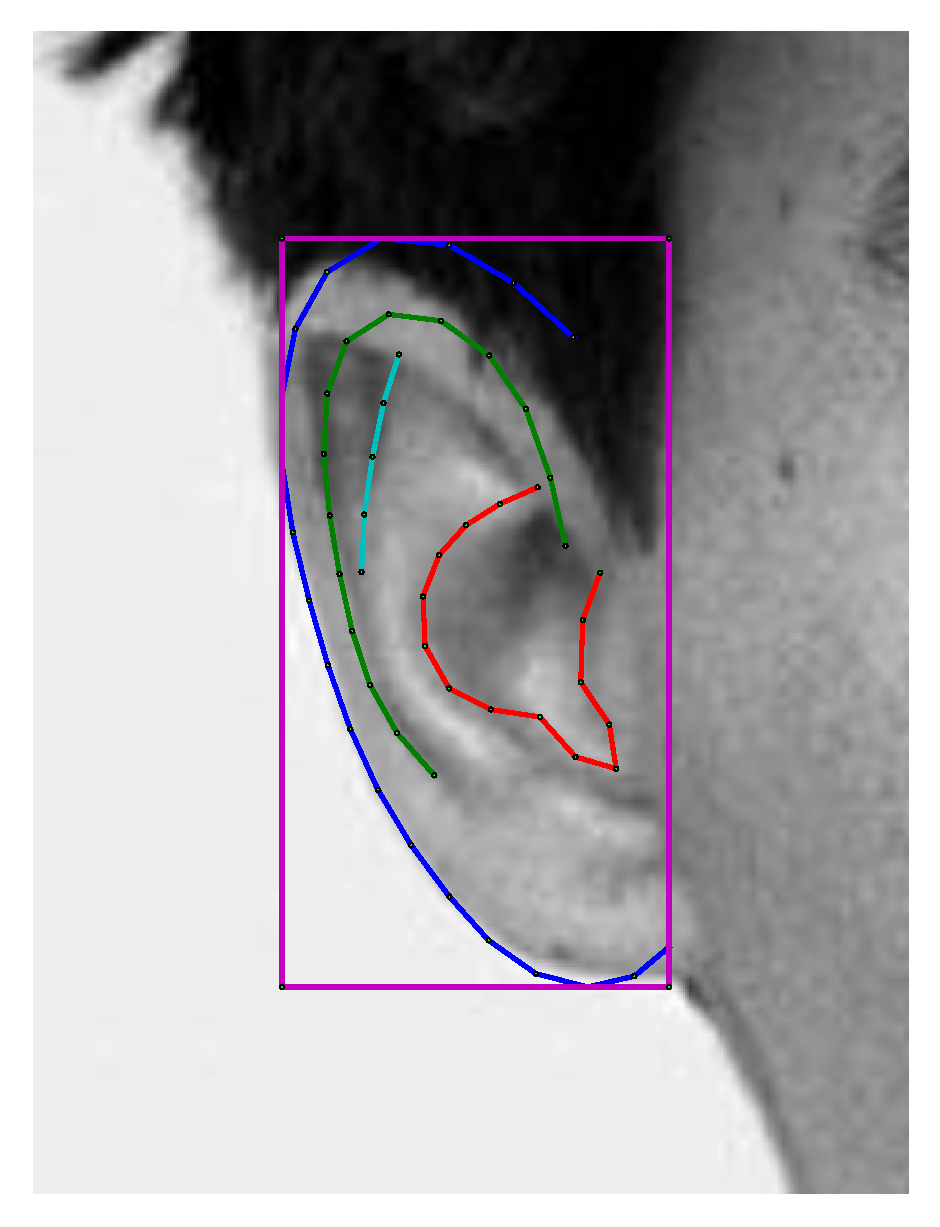
\includegraphics[height=\flowhh]{resources/Ear_Deformable_Model/fittings/initial_0020}
    % 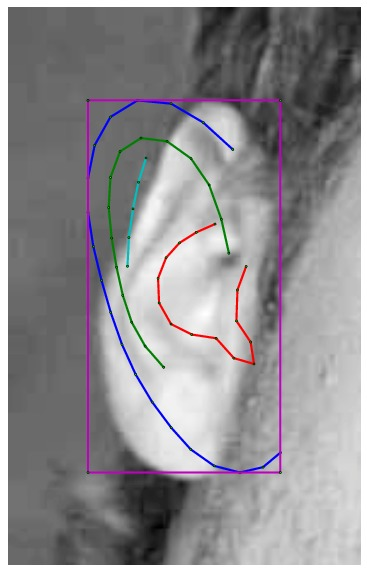
\includegraphics[height=\flowhh]{resources/Ear_Deformable_Model/fittings/initial_0026}
    % 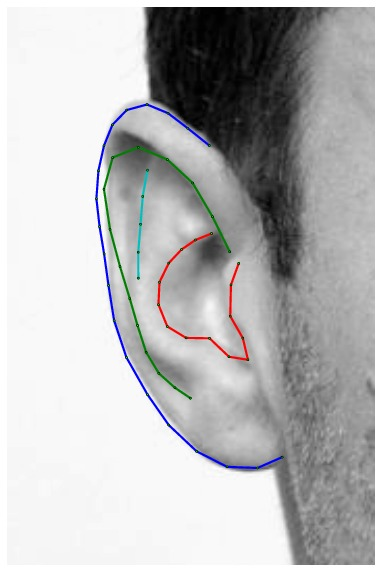
\includegraphics[height=\flowhh]{resources/Ear_Deformable_Model/fittings/final_0025}
    % \includegraphics[height=\flowhh]{resources/Ear_Deformable_Model/fittings/final_0010}
    % \includegraphics[height=\flowhh]{resources/Ear_Deformable_Model/fittings/final_0027}
    % \includegraphics[height=\flowhh]{resources/Ear_Deformable_Model/fittings/final_0020}
    % \includegraphics[height=\flowhh]{resources/Ear_Deformable_Model/fittings/final_0026}
    
    \caption{Visualisation of Holistic AAM ear fitting results (cropped to ear only for better visualisation). First row demonstrates the bounding box generated from our in-house ear detector with corresponding initialisation. Second row presented the final fitting using Holistic AAM. Figure best viewed by zooming in.}
    \label{fig:fitting_visualise}
\end{figure}


\noindent\textbf{Alternating Minimisation}
As the expression revealed, there are two variables contained ($\bm{p}$ and $\bm{\lambda}$) so it is of importance to minimise them simultaneously. As there is no dependency between AAM shape and appearance, solving $\bm{p}$ and $\bm{\lambda}$ alternatively is used by IC Algorithm. Cost functions corresponding to $\bm{\Delta p}$ and $\bm{\Delta \lambda}$ are:
% Considering creating a linear subspace, which is spanned by collection of appearance component vector $A_i$, denoted as $span(A_i)$ and $span(A_i)^\perp$ as orthogonal complement subspace. Therefore \ref{eq:aamfitting_ear} can be rewrite as:
\begin{align}
    \label{eq:aamfittingappearancevariance_ear}
    & \argmin_{\bm{\Delta p}}||\bm{T}(\mathcal{W}(\bm{p}))-\bm{a_\lambda}\mathcal{W}(\bm{\Delta p})||^2_{\bm{\hat{U}_A}} \\
    & \argmin_{\bm{\Delta\lambda}}||\bm{T}(\mathcal{W}(\bm{p}))-\bm{a_{\lambda+\Delta \lambda}}\warp{\deltap})||^2
\end{align}

where $||.||^2_{\bm{\hat{U}_A}}$ denotes vector projected into subspace $\bm{\hat{U}_A}$, which is orthogonal complements of appearance $\bm{\hat{U}_A}=\bm{I}-\bm{U_A} \bm{U_A}^T$. Because norm considers only orthogonal components of subspace, so any other components lies in $\bm{\hat{U}_A}$ can be dropped. So the optimisation is accomplished by (1) fixing appearance parameter $\bm{\lambda}$ to compute $\bm{\Delta p}$ (2) then, similarly, fixing shape parameter $\bm{p}$ to compute $\bm{\Delta\lambda}$. By given estimation of $\bm{\lambda}$, we can solve $\Delta p$ in closed form as: 
\begin{equation}
    \label{eq:dpic_ear}
    \bm{\Delta p}=\bm{H}^{-1}\bm{J}^T[\bm{T}(\mathcal{W}(\bm{p}))-\bm{\bar{a}}-\bm{U_A}\bm{\lambda}]
\end{equation}
where $\bm{H}$ is the Hessian matrix $\bm{H}=\bm{J}^T\bm{J}$. Given estimation of $\bm{p}$, appearance parameters can be solved as least-squares solution:
\begin{equation}
    \label{eq:lambdaic}
    \bm{\Delta \lambda}=\bm{U_A^T}[\bm{T}(\mathcal{W}(\bm{p}))-\bm{\bar{a}}(\mathcal{W}(\bm{\Delta p}))-\bm{U_A}(\mathcal{W}(\bm{\Delta p}))\bm{\lambda}]
\end{equation}
where appearance parameters are updated by $\bm{\lambda}\leftarrow\bm{\lambda}+\bm{\Delta \lambda}$. 

As the equation states, image template $\bm{\bar{a}}$ is constant and the gradient of warp $\frac{\partial \mathcal{W}}{\partial \bm{p}}$ is always evaluated at appearance template, which remains constant. Therefore Jacobian at initial iteration and Hessian Matrix $\bm{H}$ can be precomputed before optimising cost function.


\subsection{Patch-based Active Appearance Model} 
The difference between a holistic and a patch-based AAM~\cite{Tzimiropoulos2014} is on the way that the appearance vectors are extracted, as well as the deformation model. As explained in the previous section, a holistic appearance is retrieved using the warp function in order to map the locations of all the pixels of a given shape into a common reference shape and transfer their values. However, under a patch-based formulation, this procedure is greatly simplified and an appearance vector is acquired by concatenating the features (e.g. SIFT) extracted from the patches centred at the landmarks of a provided shape instance. Thus, the affine warp function is replaced by a simple sampling function. In~\cite{Tzimiropoulos2014} it is shown that due to this difference, the compositional update of the shape parameters becomes additional, i.e. $\mathbf{p}\leftarrow\mathbf{p} + \Delta\mathbf{p}$. The rest of the Gauss Newton optimisation remains the same.

Patch-based AAMs achieve more accurate performance compared to holistic AAMs on the task of face alignment~\cite{Tzimiropoulos2014}. However, this is easily explained by the fact that the inner appearance information of a human face (i.e. cheeks eta.) does not have a distinctive structure. Experiment \ref{sec:ear_benchmark_fitting} further explains the advanced performance of holistic AAM on ears where inner appearance is complex and rich. In general, the selection of a holistic or patch-based appearance representation highly depends on the nature of the modelled object and its interior structure. 

\subsection{Dense Active Appearance Model}
TODO

\section{3D Morphable Models for Ears}
TODO


%%%%%%%%%%%%%%%%%%%%%%%%%%%%%%%%%%%%%%%%%%%%%%%%%%%%%%%%%%%%%%%%%%%%%%%%%%%%%%%%


\section{Experimental Evaluation}

We have conducted two set of extensive experiments. The first set of experiments concerns ear landmark localisation using the Collection A. The second set of experiments revolves around ear recognition/verification using Collection B. In particular, the aim and motivation of ear recognition/verification experiments are the following. (a) To demonstrate the shortcomings of the current available databases, and particular WPUTEDB, (b) to demonstrate the challenges that emerge from our new database and (c) to demonstrate the effect of alignment in recognition/verification.  


% ----------------------------------------------------------------------------------------------------------------

\begin{figure}
\centering
\newcommand{\flowh}{0.29\columnwidth}
    \centering
    \includegraphics[height=\flowh]{resources/Ear_Deformable_Model/ear_02}
    \hfill
    \includegraphics[height=\flowh]{resources/Ear_Deformable_Model/ear_10}
    \hfill
    \includegraphics[height=\flowh]{resources/Ear_Deformable_Model/ear_14}
    \hfill
    \includegraphics[height=\flowh]{resources/Ear_Deformable_Model/ear_24}
\caption{Examplar visualisations showing different values of normalised point-to-point error measure for ears (0.06, 0.10, 0.14, 0.24 respectively). Figure best viewed by zooming in.}
\label{fig:ear_error}
\end{figure}


\subsection{Ear Fitting Evaluation}
\label{sec:ear_benchmark_fitting}

We evaluated the performance of many state-of-the-art methodologies including AAM, CLM and SDM using various kind of features. In particular, we employed pixel intensity (PI), dense SIFT (DSIFT)~\cite{lowe1999object}, dense HOG~\cite{Dalal2005}, IGO~\cite{tzimiropoulos2012subspace} and DCNN~\cite{sermanet2013overfeat} features for both holistic and patch-based AAMs. The models were trained on a 3-level Gaussian pyramid. We kept $[3, 6, 12]$ shape components for each level (low to high) and $90\%$ of the appearance variance for all levels. Also discriminative models like Supervised Descend Method (SDM)~\cite{xiong2013supervised} and Constrained Local Model (CLM)~\cite{cristinacce2006feature}  are involved using features DSIFT~\cite{lowe1999object}. Figure~\ref{fig:aam_model} visualises the first five shape and appearance principal components of the holistic AAM and, as it can be observed, the variation of both shape and appearance is plausible. Appearance components are shown using pixel intensities for better visualisation. Note that any technologies involved in this paper was implemented using the Menpo Platform~\cite{alabort2014menpo}.

For all the tested methods we computed the Cumulative Error Distribution (CED) curves which is the standard way of visualising the performance of deformable models. The fitting error is computed using the point-to-point error normalised by the diagonal of the ear's bounding box that tightly bounded ground truth annotations, as proposed in~\cite{Zhu2012}.


\begin{figure}
    \centering
    \includegraphics[width=\columnwidth]{resources/Ear_Deformable_Model/benchmark_ear_legend} \\
    \includegraphics[width=\columnwidth]{resources/Ear_Deformable_Model/benchmark_ear}
    \caption{Experimental results on our testing 121 dataset evaluated on 55 landmarks. Fitting accuracy reported for Holistic AAM, patch-based AAM, SDM and CLM.}
    \label{fig:fitting_results}
\end{figure}

\begin{table}
\small
\centering
\begin{tabular}{|l|c|c|c|}
\hline
\emph{Method}   & \emph{mean $\pm$ std} & \emph{median} & $\leq 0.10$\\
\hline\hline
DCNN+AAM & 0.0599 $\pm$ 0.0272  & 0.0542 & 93\%\\
SIFT+AAM & $\bm{0.0522}$ $\pm$ $\bm{0.0246}$  & $\bm{0.0453}$ & 94\%\\
HOG+AAM & 0.0539 $\pm$ 0.0248  & 0.0479 & $\bm{97\%}$ \\
IGO+AAM & 0.0786 $\pm$ 0.0295  & 0.0738 & 77\%\\
PI+AAM & 0.2124 $\pm$ 0.2674  & 0.1342 & 36\%\\
\hline
SIFT+PAAM & 0.0563 $\pm$ 0.0264  & 0.0493 & 93\%\\
HOG+PAAM & 0.0860 $\pm$ 0.0533  & 0.0700 & 73\%\\
IGO+PAAM & 0.0704 $\pm$ 0.0272  & 0.0709 & 86\%\\
PI+PAAM & 0.1049 $\pm$ 0.0733  & 0.0729 & 64\%\\
\hline
SDM & 0.0890 $\pm$ 0.0348  & 0.0862 & 65\%\\
CLM & 0.0862 $\pm$ 0.0296  & 0.0830 & 81\%\\
\hline
Initialisation & 0.1276 $\pm$ 0.0332  & 0.1283 & 23\%\\
\hline
\end{tabular}
\caption{Fitting statistics on ear database Collection A}
\label{tab:ear_stats}
\end{table}


Figure~\ref{fig:fitting_results} reports the CED curves of all the tested methods along with the initialisation curve. The fitting is initialised using our own in-house ear detector based on HoG SVMs that was trained with in-the-wild ear images of the training set of Collection A. Figure~\ref{fig:ear_error} shows some characteristic examples of different error values in order to give an intuition about the fitting quality of each error bin of the CED curves, which indicates that normalised point-to-point error less or equal than 0.10 is acceptable. The figure reveals that DSIFT tends to give most representative features for ears and holistic AAMs in general outperform patch-based AAM. This is attributed to the fact that holistic texture model can represent the complex inner structure of ears in a better fashion. The poor performance of SDM could be associated to the limited annotated data, as well as to the use of a part-based texture model. 


Table \ref{tab:ear_stats} complements Figure~\ref{fig:fitting_results} by reporting some statistical metrics, i.e. the mean, median and standard deviation of the errors. Finally, Figure~\ref{fig:fitting_visualise} shows some qualitative fitting results along with their initialisations.


% ----------------------------------------------------------------------------------------------------------------



\begin{figure}
    \centering
    \newcommand{\flowhh}{0.36\columnwidth}
    \newcommand{\flowh}{0.32\columnwidth}
    \includegraphics[height=\flowhh]{resources/Ear_Deformable_Model/verification/background_exp/ear_bg_0}
    \hfill
    \includegraphics[height=\flowhh]{resources/Ear_Deformable_Model/verification/background_exp/ear_bg_1}
    \hfill
    \includegraphics[height=\flowhh]{resources/Ear_Deformable_Model/verification/background_exp/ear_bg_2}
    \\
    \includegraphics[height=\flowh]{resources/Ear_Deformable_Model/verification/background_exp/ear_bg_3}
    \includegraphics[height=\flowh]{resources/Ear_Deformable_Model/verification/background_exp/ear_bg_4}
    \includegraphics[height=\flowh]{resources/Ear_Deformable_Model/verification/background_exp/ear_bg_5}
    \caption{Exemplar visualisation of background of the ear in both the WPUTEDB, as well as the proposed database. Top row: the background of ear images of WPUTEDB for one subject. Bottom row: images of the background from the proposed database for one subject. The black area covers the ear region.}
    \label{fig:bg_exp}
\end{figure}


\begin{table}
\centering
\begin{tabular}{|l|c|c|}
\hline
& WPUTEDB & Our Database\\
& \emph{mean $\pm$ std} & \emph{mean $\pm$ std} \\
\hline\hline
\multicolumn{3}{|l|}{Aligned}\\
\hline

LDA+PI              &  0.6581 $\pm$ 0.0030 &       0.2272 $\pm$ 0.0169 \\
LDA+HOG+PCA         &  0.8195 $\pm$ 0.0058 &       0.5123 $\pm$ 0.0162 \\
LDA+DSIFT+PCA       &  0.8082 $\pm$ 0.0098 &       0.5496 $\pm$ 0.0180\\
LDA+PPSIFT+PCA      &  $\bm{0.9076}$ $\pm$ $\bm{0.0038}$ &       $\bm{0.6684}$ $\pm$ $\bm{0.0195}$\\

\hline\hline
\multicolumn{3}{|l|}{Unaligned}\\
\hline

LDA+PI              &  0.5993 $\pm$ 0.0025 &       0.1429 $\pm$ 0.0123\\
LDA+HOG+PCA         &  $\bm{0.7784}$ $\pm$ $\bm{0.0074}$ &       0.3250 $\pm$ 0.0105\\
LDA+DSIFT+PCA       &  0.7621 $\pm$ 0.0082 &       $\bm{0.3348}$ $\pm$ $\bm{0.0138}$\\

\hline\hline
\multicolumn{3}{|l|}{Background Only}\\
\hline

LDA+DSIFT+PCA       &  0.5676 $\pm$ 0.0312 &       0.0827 $\pm$ 0.0173 \\
\hline
\end{tabular}
\caption{Ear Recognition experiments on WPUTEDB and the proposed database. Multiple features and classification algorithms are applied with/without alignment.}
\label{tab:ear_recognition}
\end{table}



\subsection{Ear Recognition Experiments}


%In general, ear recognition using training and testing images are normalised and contained within tight bounding boxes. Assume that their exist $x_1,x_2,...,x_m \in R^n$ images of size $n$. With general ear recognition algorithms, $n$ are defined as $n=width\times height \times n_{channels}$ where width and height are corresponding size of bounding boxes and are normalized to have exactly same size for each $x_m$. $n_{channels}$ are depends on images features, e.g. 1 channel for intensity, 3 channels for RGB images and more for SIFT and HOG. 

In order to conduct close ear recognition experiments we conducted a 10 fold cross validation experiment where 90$\%$ were used for training  and 10$\%$ testing in each fold. We report average accuracy and standard deviation. In order to compare how challenging each database is we applied the above protocol to both our database, as well as WPUTEDB, which contains largest amount of subjects and most significant appearance variance among existing ear databases but still collected under controlled environment. Furthermore, we wanted to investigate how the background of the ear images of WPUTEDB biases the results, since from Figure \ref{fig:bg_exp} it is evident that the background is very similar in the ear images of the same person of WPUTEDB.

Classification of ears was implemented by applying generic classification pipelines. In particular, the we applied the standard pipeline of feature extraction + dimensionality reduction + multi-class classification. For features we explored pixel intensities, HOG, SIFT and Pyramid Patch SIFT (PPSIFT) \footnote{To compute PPSIFT, we build image pyramid for given images by rescale it by 0.25, 0.5, 1.0 of original image including landmarks. Then we extract small patches around landmarks at each pyramid level and compute SIFT feature so each patch gives a vector of size 128. PPSIFT are constructed by concatenating all patches.}. For dimensionality reduction we used a Principal Component Analysis plus Linear Discriminant Analysis (PCA plus LDA) framework~\cite{belhumeur1997eigenfaces}. For classification we using a multi-class SVM~\cite{hsu2002comparison}.


Finally, we compared aligned versus non-aligned ears. For alignment we used the previously described SIFT+AAM framework to locate the landmarks. We applied the AAM deformation model warp function to map all the points to the reference shape. This procedure is necessary in order to bring the SIFT features appearance vectors of all fitted images into correspondence. We employ the Piecewise Affine Warp, which performs the mapping based on the barycentric coordinates of the corresponding triangles between the two shapes that are extracted using Delaunay Triangulation. For the non-aligned version of experiments we used the cropped ear images from the detected bounding box. In both cases the ear images were rescaled in a $200 \times 200$ bounding box before feature extractions. 

From the results reported in Table \ref{tab:ear_recognition} we can deduce the following (a) the collected database is far more challenging than the WPUTEDB, (b) the background around the ear does not play any role in the proposed database, while the background gives a 57$\%$ recognition rate in WPUTEDB \footnote{Since images from WPUTEDB for each subjects are all collected in short periods, even background (e.g. hair and earrings) provides significant support to classification which is not the case in our database.}, (c) the alignment largely improves performance (approximately 5\% average in WPUTEDB and 10\% to 20\% in our database) and (d) the best performance is achieved by PPSIFT features. 

% ----------------------------------------------------------------------------------------------------------------
\afterpage{
    \begin{figure}
    \centering
    % \newcommand{\floww}{0.49\columnwidth}
    \includegraphics[width=\columnwidth]{resources/Ear_Deformable_Model/verification/verification_bench_label}
    \\
    \includegraphics[width=0.45\columnwidth]{resources/Ear_Deformable_Model/verification/verification_bench_aligned}
    \hfill
    \includegraphics[width=0.45\columnwidth]{resources/Ear_Deformable_Model/verification/verification_bench_unaligned}
    \caption{ROC curves averaged over 5 folds on the proposed database (top: using aligned images, bottom: using unaligned images).}
    \label{fig:ear_benchmark}
    \end{figure}
    
    \begin{table}
    \centering
    
    \begin{tabular}{|l|c|c|}
    \hline
    
                            &   Aligned             &   Unaligned  \\
    \emph{Method}    & \emph{mean $\pm$ std} & \emph{mean $\pm$ std} \\
    \hline\hline
    PI+LDA           & 0.5659 $\pm$ 0.017    & 0.5405 $\pm$ 0.023 \\
    DSIFT+PCA+LDA    & 0.6222 $\pm$ 0.012    & 0.6178 $\pm$ 0.025 \\
    JBC+EigenPEP+PCA & 0.6297 $\pm$ 0.013    & 0.6189 $\pm$ 0.023 \\
    DCNN+LDA         & $\bm{0.6859}$ $\pm$ $\bm{0.024}$    & 0.6492 $\pm$ 0.032 \\
    \hline
    \end{tabular}
    \caption{Ear verification benchmark on Collection B. Mean and variance of verification accuracy are reported for a set of methods applying on both aligned and unaligned data.}
    \label{tab:ear_verification_benchmark}
    \end{table}
}


\subsection{Ear Verification Experiments}

In this section we have designed and executed an ear verification experiment reminiscent of the experimental protocol of Labelled Faces in-the-wild (LFW)~\cite{huang2007labeled}.  That is, evaluation is performed by determining whether a pair of images come from the same person or not. In the case of ear verification, 185 positive and 185 negative matching pairs are generated for each fold and total five folds are generated, from which we perform a leave-one-out cross validation.

We used similar features as in the recognition experiments. In particular, we applied pixel intensities (PI), DSIFT and Deep Convolutional Neural Networks (DCNN)~\cite{simonyan2014very} (for DCNN we used the pre-trained VGG-16 architecture). High dimensional features, such as DSIFT, were combined with PCA for dimensionality reduction. For each pair of the training images and for each feature we computed the squared distance and formed a vector which was fed to a two class LDA or SVM which separate match versus not-match pairs. We apply the above methods to both aligned and non-aligned ear samples. Finally, we also applied the methodology that was proposed in~\cite{li2014eigen} (so-called Eigen-Pep).


Overall performance over five folds is reported using mean accuracy (as in LFW). Experiments are performed under the image-restricted setting, where only binary positive or negative labels are given, for pairs of images. So the identity information of each image is not available under this setting and results are reported with both no outside training data and label-free outside data for alignment. Table \ref{tab:ear_verification_benchmark} summarises the results. The top performance is around 68$\%$ using DCNN features and aligned images. As in the recognition experiments alignment always improves performance. Finally, Figure  \ref{fig:ear_benchmark} plots the ROC curves for the tested methods.


%\subsubsection{Inter and Intra database experiments}

%We conducted a final set of experiments in order to measure the discriminant information of the proposed database over WPUTEDB. 
%In particular, we conducted a series of inter and intra database experiments. First we applied a 5-fold split of WPUTEDB. Then, we used the training set of WPUTEDB to train the classifier of match and non-match and tested on the proposed database and vice-versa. 


%\begin{figure}[!t]
%\centering
%% \newcommand{\floww}{0.49\columnwidth}
%\includegraphics[width=\columnwidth]{resources/Ear_Deformable_Model/verification/verification-comp-label}
%\\
%\includegraphics[width=\columnwidth]{resources/Ear_Deformable_Model/verification/verification-comp-align}
%\\
%\includegraphics[width=\columnwidth]{resources/Ear_Deformable_Model/verification/verification-comp-unalign}


%\caption{ROC curves averaged over 5 folds of between database experiments (top: aligned, bottom unaligned).}
%\label{fig:ear_compare}
%\end{figure}

%\begin{table}[!t]
%\centering
%\scriptsize
%\begin{tabular}{|l|c|c|c|c|c|c|}
%\hline
%Method             &  $W_{r}$ & $W_{a}$ &  $P_{r}$ & $P_{a}$  &$W_r-W_a$&  $P_r-P_a$  \\
%\hline\hline
%\multicolumn{7}{|l|}{aligned}\\
%\hline
%LDA+PI              & 0.6768 & 0.5773 & 0.5605 & 0.6562 &  0.0957 &  0.0995 \\
%SVM+PI              & 0.6573 & 0.5724 & 0.5568 & 0.6476 &  0.0908 &  0.0849 \\
%LDA+DSIFT           & 0.6541 & 0.5886 & 0.6222 & 0.6389 &  0.0168 &  0.0654 \\
%SVM+DSIFT           & 0.6389 & 0.5638 & 0.6032 & 0.5811 & -0.0222 &  0.0751 \\
%\hline\hline
%\multicolumn{7}{|l|}{unaligned}\\
%\hline
%LDA+PI              & 0.6465 & 0.5492 & 0.5659 & 0.5708 &  0.0049 &  0.0973 \\
%SVM+PI              & 0.6270 & 0.5486 & 0.5270 & 0.6000 &  0.0730 &  0.0784 \\
%LDA+DSIFT           & 0.6454 & 0.5865 & 0.6189 & 0.6373 &  0.0184 &  0.0589 \\
%SVM+DSIFT           & 0.6238 & 0.5546 & 0.6092 & 0.5876 & -0.0216 &  0.0692 \\
%\hline
%\end{tabular}


%\caption{Ear verification on WPUTEDB (W) and the proposed database (P). Verification accuracy reported for both databases under %inter-database verifications and cross-database verification.}
%\label{tab:ear_verification}
%\end{table}

%\noindent\textbf{Results}
%Table~\ref{tab:ear_verification} presented ear verification accuracy between WPUTEDB(W) and our database(P), where $A_d$ and $B_d$ represent "direct" verification that training and testing are performed within same dataset s, while $A_c$ and $B_c$ means "cross" verification that training and testing happened between different datasets. Corresponding ROC plots can be found in figure~\ref{fig:ear_compare}.

%As for "direct" verification (taking $A_d$ and $B_d$ into account), WPUTEDB reported higher verification accuracy in all methods as expected. Also images with AAM alignment improves accuracy for notable amount. The highest verification achieved are 68\% and 62\% respectively. 

%In the case of between database verification, for each validation fold, test set are swapped so algorithm are trained on training set from one database but tested on the test set of the other. Here we focus on the performance difference for the same method trained on one training set but tested on different test sets, which refers to $A_d-A_c$ and $B_c-B_d$ on both database. As the results shown, models trained on $A$ are not general enough to cope with the test set from $B$ according to high $A_d-A_c$ value, which is around 8\% difference. In contrast, the same model trained on B is more robust against testing data from A and, in most case, reported verification accuracy improvement subjects to $B_c-B_d$ value and marginal performance reduction in worst cases. 

%Table~\ref{tab:ear_verification_benchmark} and figure~\ref{fig:ear_benchmark} reported baseline of ear verification on our database. In general, ear verification with AAM frontalisation gives better performance. The methods reported highest verification accuracy (around 69\%) are LDA trained on DCNN feature with $\ell_2^2$ norm.


\subsection{Dense Ear Landmark Regression}
\label{sec:exp_ear}

TODO: link to next chapter

We have also performed experiments on the human ear. We employ the $605$ images and sparse landmark annotations that were generated in a semi-supervised manner by Zhou et al.~\cite{Zhou_2016_CVPR}. Due to the lack of a 3D model of the human ear, we apply Thin Plate Splines to bring the images into dense correspondence and obtain the deformation-free space. We perform landmark localization following the same procedure as in Sec.~\ref{sec:exp_landmark_localization}.
We split the images in $500$ for training and $105$ for testing.  


Given the lack of state-of-the-art deformable models on human ear, we compare DenseReg with DenseReg+AAM and DenseReg+MDM.  We also trained a DPM detector in order to compare the initialization quality with DenseReg. Figure~\ref{fig:ears} reports the CED curves based on the 55 landmark points using the RMS point-to-point error normalized by the bounding box average edge length. On Table.\ref{tab:ears}, we provide failure rate and the Area Under Curve(AUC) measures. Once again, the results are highly accurate even without improving DenseReg with a deformable model. We observe that DenseReg results are highly accurate and clearly outperforms the DPM based alternative even without a deformable model. Examples for dense human ear correspondence estimated by our system  are presented in Fig.~\ref{fig:ears_examples}.


\begin{figure}
\centering
\includegraphics[width=\linewidth]{resources/Ear_Deformable_Model/dense/ears3.pdf}
\caption{Exemplar pairs of deformation-free coordinates of dense landmarks on human ear.}
\vspace{-0.5cm}
\label{fig:ears_examples}
\end{figure}


\begin{figure}
\centering
\includegraphics[width=\linewidth]{resources/Ear_Deformable_Model/dense/ear_legend.pdf}
\includegraphics[width=\linewidth]{resources/Ear_Deformable_Model/dense/ear_results.pdf}
\caption{Landmark localization results on human ear using 55 points. Accuracy is reported as Cumulative Error Distribution of normalized RMS point-to-point error.}
\vspace{-0.25cm}
\label{fig:ears}
\end{figure}


%%%%%%%%%%%%%%%%%%%%%%%%%%%%%%%%%%%%%%%%
% \FloatBarrier
\begin{table}
\centering
\begin{tabular}{|l|c|c|}
\hline
\emph{Method} & \emph{AUC} & \emph{Failure Rate (\%)}\\
\hline\hline
\textbf{DenseReg + MDM} & \textbf{0.4842} & \textbf{0.98} \\
DenseReg       &  0.4150 &   1.96 \\
DenseReg + AAM &  0.4263 &  0.98 \\
DPM + MDM      &  0.4160 &  15.69 \\
DPM + AAM      &  0.3283 &  22.55 \\
\hline
\end{tabular}
\caption{Landmark localization results on human ear using 55 points. Accuracy is reported as the Area Under the Curve (AUC) and the Failure Rate of the Cumulative Error Distribution of the normalized RMS point-to-point error.}
\label{tab:ears}
\end{table}


%%%%%%%%%%%%%%%%%%%%%%%%%%%%%%%%%%%%%%%%%%%%%%%%%%%%%%%%%%%%%%%%%%%%%%%%%%%%%%%%
\section{Conclusion}
In this paper, we collected two sets of challenging in-the-wild ear databases for the purpose of ear deformable model constructions and ear recognition/verification. The experimental evaluation and comparison revealed that holistic and patch-based AAMs can align images of ears captured ``in-the-wild''. We conducted extensive recognition and verification experiments. The experiments convincingly  demonstrate that (a) the proposed database is very challenging and (b) alignment consistently improves performance.